\documentclass[11pt,a4paper]{article}

\usepackage{iftex}
\usepackage{amsthm}
\usepackage{amsmath,amssymb}
\ifPDFTeX
  \usepackage[T2A]{fontenc}
  \usepackage[utf8]{inputenc}
\else
  % XeLaTeX / LuaLaTeX (в т.ч. tectonic): Unicode-шрифт с кириллицей
  \usepackage{fontspec}
  \setmainfont{Times New Roman}
\fi
\usepackage[russian,english]{babel}
\usepackage[margin=2.3cm]{geometry}
\usepackage[hidelinks]{hyperref}
\usepackage{xcolor}
\usepackage{graphicx}
\usepackage{booktabs}
\usepackage{tabularx}

\setlength{\emergencystretch}{2em}
\newcommand{\todo}[1]{\textcolor{red}{[TODO: #1]}}
% обзор литературы — один раздел с подразделами
\newcommand{\RWsection}{\subsection}
\newcommand{\RWsubsection}{\subsubsection}

\title{Детерминированные алгоритмы аппроксимации первых слоёв LLM}
\author{\todo{авторы}}
\date{}

\begin{document}
\selectlanguage{russian}
\maketitle

\begin{abstract}
\newtheorem{proposition}{Предложение}
% Аннотация (подключается в annotation.tex и main.tex)
Первые слои больших языковых моделей (LLM) на основе архитектуры
Transformer~\cite{vaswani2017attention} выполняют сравнительно простые
операции: восстанавливают статистику биграмм и коротких
$n$-грамм~\cite{elhage2021framework}, реализуют фиксированные позиционные
паттерны внимания и хранят поверхностные шаблоны в слоях
прямого распространения~\cite{geva2021ffn}.
Мы исследуем гипотезу о том, что вычисления первых $k$ слоёв можно
заменить \emph{детерминированными} алгоритмами, то есть процедурами без
случайной выборки и без дообучения градиентным спуском, которые
строятся по весам модели и статистике калибровочного корпуса в
замкнутой форме. Мы адаптируем к каузальному декодеру Qwen3 методы
эффективного внимания и сжатия слоёв MLP из литературы и предлагаем
собственные: факторизацию внимания <<позиционное ядро $\times$
значимость ключевого токена>>, типизированную замену голов,
линеаризацию MLP с компенсацией дрейфа остаточного потока и табличные
замены блоков. Эксперименты проводятся на Qwen3-0.6B и 1.7B
(Base) с оценкой по KL-дивергенции к исходной модели, perplexity и
стандартным бенчмаркам.
Профилирование показывает, что первые слои образуют отдельный режим
<<до стока внимания>>: массивная активация первого токена и сток
внимания возникают лишь после нескольких первых слоёв, что задаёт
естественную глубину замены $k_{\mathrm{sink}}$. Мы также показываем,
что рандомизированные признаки FAVOR+ (Performer~\cite{choromanski2021performer})
неприменимы к первым слоям без переобучения: нормы ключей после
QK-нормализации лежат далеко за пределами области, где их оценка
ядра устойчива.
Основные результаты. (1) Внимание первых трёх слоёв заменяется окном
из 64 позиций со стоком с ростом perplexity 1.5--1.8\,\% и без потерь на
семи бенчмарках; MLP первых слоёв заменяется хуже: лучший метод "---
предложенный детерминированный предиктор активных нейронов "--- стоит
4.7\,\% (0.6B) и 1.7\,\% (1.7B) при четверти вычислений MLP, а по карте
заменяемости MLP ранних слоёв оказываются самыми незаменимыми в модели.
(2) Мы обнаруживаем ловушку калибровки в замкнутой форме: единичные
токены с массивной активацией доминируют в задаче наименьших квадратов,
ошибка ложится в каналы стока внимания и обрушивает модель; мы даём
формулу влияния строки, воспроизводим эффект дозой отравленных окон и
устраняем его исключением строк-выбросов, а также показываем, что
массивную активацию создают один--пять нейронов, удаление которых
разрушает модель. (3) Априорные статистики слоя предсказывают KL его
замены с ранговой корреляцией 0.9--0.97 и позволяют планировать замены
на непросмотренной модели в 10--15 раз точнее замены префикса.
(4) На втором семействе (SmolLM2-1.7B, Llama-3.2-1B) сток оказывается
привязан не к позиции, а к токену: один нейрон создаёт массивную
активацию на <<the>> в любой позиции, и замены переносятся лишь с
защитой таких нейронов и хранением таких ключей (окно: $64\to4\,\%$ PPL
при $k=8$); MLP первых слоёв у этого семейства заменяется хуже, а
планировщик переносится.
Результаты дополняют дискуссию о том, насколько внутренние вычисления
обученных сетей <<уже чисты>> и поддаются явному
описанию~\cite{cammarata_clean,gao_notclean}.

\medskip
\noindent\textbf{Ключевые слова:} трансформеры, большие языковые модели,
аппроксимация внимания, механистическая интерпретируемость,
детерминированные алгоритмы, низкоранговые приближения, сжатие MLP.

\end{abstract}

% Введение (подключается в annotation.tex и main.tex)
\section{Введение}

Архитектура Transformer~\cite{vaswani2017attention} стала основой
современных больших языковых моделей. Её центральный механизм,
самовнимание (self-attention), требует $O(n^2)$ операций по длине
последовательности $n$. Это породило большое семейство методов
эффективной аппроксимации внимания. Их можно условно разделить на
несколько групп:
\begin{itemize}
  \item \textbf{ядерные и линейные} методы, в которых softmax заменяется
    скалярным произведением признаковых отображений: линейное
    внимание~\cite{katharopoulos2020rnn}, Performer со случайными
    признаками FAVOR+~\cite{choromanski2021performer}, случайные
    фурье-признаки RFA~\cite{peng2021rfa}, SOFT без
    softmax~\cite{lu2021soft};
  \item \textbf{низкоранговые} методы: проекции Linformer по оси
    последовательности~\cite{wang2020linformer}, приближение Нистрёма
    в Nyströmformer~\cite{xiong2021nystrom}, аналитический фреймворк
    A3~\cite{wong2025a3};
  \item \textbf{разреженные} шаблоны внимания: Sparse
    Transformer~\cite{child2019sparse}, хеширование LSH в
    Reformer~\cite{kitaev2020reformer}, комбинация локального,
    глобального и случайного внимания в BigBird~\cite{zaheer2020bigbird};
  \item \textbf{замена внимания} фиксированным или
    синтезированным смешиванием токенов: преобразование Фурье в
    FNet~\cite{leethorp2022fnet}, Synthesizer~\cite{tay2021synthesizer}.
\end{itemize}

Почти все эти методы аппроксимируют механизм внимания \emph{равномерно
по глубине}: одна и та же схема применяется во всех слоях и, как
правило, требует обучения модели с нуля или дообучения. При этом
многие из них по своей природе \emph{стохастичны}: случайные признаки,
случайные хеш-функции, случайные рёбра графа внимания. Из-за этого
ошибка аппроксимации зависит от выборки, а результат вычислений
воспроизводим лишь с точностью до зерна генератора.

Параллельно развивается механистическая интерпретируемость: она
показывает, что слои трансформера неоднородны по своей
функции~\cite{olah2020zoom,rai2024review}. Математический анализ
трансформерных схем~\cite{elhage2021framework} показывает, что модель
без слоёв внимания приближает статистику биграмм. Однослойная модель,
состоящая только из внимания, дополнительно реализует
<<skip-trigram>>-зависимости. Индукционные головы, которые
обеспечивают обучение в контексте, возникают лишь при композиции как
минимум двух слоёв внимания~\cite{olsson2022induction}. Слои прямого
распространения работают как память <<ключ--значение>>, причём ключи
нижних слоёв реагируют на поверхностные шаблоны (конкретные
$n$-граммы), а верхних "--- на семантические~\cite{geva2021ffn}.
Словарное обучение на активациях MLP небольшой модели выделяет
интерпретируемые моносемантические признаки~\cite{bricken2023monosemanticity}.
Известно также, что многоголовое самовнимание способно выражать
свёрточные слои~\cite{cordonnier2020relationship}. Значит, локальные
позиционные паттерны внимания в принципе описываются фиксированными
ядрами. Наконец, теоретический анализ
показывает, что чистое внимание без остаточных связей и MLP
вырождается по рангу дважды экспоненциально с
глубиной~\cite{dong2021attention}. Поэтому остаточный поток играет
ключевую роль при любой послойной замене вычислений.
Отдельно идёт дискуссия о том, являются ли обученные нейросети
<<уже чистыми>> (\emph{already clean}), то есть поддающимися явному
описанию~\cite{cammarata_clean,gao_notclean,lissack_clean,ibm_clean}.
Cammarata~\cite{cammarata_clean} утверждает, что видимая
полисемантичность нейронов в основном объясняется не суперпозицией, а
<<рекурсивным обобщением>> связанных понятий, и по предварительной
оценке около 90\% <<полюсов>> нейронов Qwen3-32B (положительная или отрицательная сторона активации) имеют одну основную функцию.
Gao~\cite{gao_notclean} возражает, что совпадения активирующих примеров с
шаблоном недостаточно, и предлагает строгий критерий: объяснение
верно, если подстановка смоделированных по нему активаций не
увеличивает KL-дивергенцию выходного распределения модели. Именно этот
критерий "--- KL при подстановке "--- мы используем как основную
метрику замены слоёв.

Эти наблюдения подсказывают иную постановку задачи. Если первые слои
LLM реализуют в основном локальные, <<поверхностные>> вычисления, то
их можно заменить \emph{явными детерминированными алгоритмами} вместо
единообразной аппроксимации внимания во всей сети. Под
детерминированным алгоритмом мы понимаем процедуру, которая
\begin{enumerate}
  \item не использует случайную выборку на этапе вывода;
  \item строится по весам обученной модели и/или статистике корпуса
    в замкнутом виде или явной процедурой, без градиентного
    дообучения;
  \item даёт одинаковый выход на одинаковом входе и допускает
    аналитическую оценку ошибки.
\end{enumerate}
Примеры таких алгоритмов: фиксированные разреженные шаблоны внимания,
позиционные ядра вместо голов внимания, таблицы поиска по токенам,
аналитические низкоранговые разложения матриц $W_{QK}$, $W_{OV}$ и
весов MLP~\cite{wong2025a3,yuan2023asvd,wang2025svdllm}, линейные
карты, подогнанные гребневой регрессией.

\paragraph{Постановка задачи.}
Пусть $f = f_L \circ \dots \circ f_1 \circ E$ "--- языковая модель из
$L$ блоков с матрицей эмбеддингов $E$, а $h_k(x)$ "--- состояние
остаточного потока после $k$-го блока на входе $x$. Требуется
построить детерминированный алгоритм $A_k$, такой что
\[
  \tilde f = f_L \circ \dots \circ f_{k+1} \circ A_k,
  \qquad
  \mathbb{E}_{x}\,
  \mathrm{KL}\bigl(p_f(\cdot \mid x)\,\|\,p_{\tilde f}(\cdot \mid x)\bigr)
  \le \varepsilon,
\]
и определить максимальную глубину $k^{*}(\varepsilon)$, для которой
это возможно при ограничениях на вычислительную сложность и память
алгоритма $A_k$.

\paragraph{Вклад работы.}
\begin{enumerate}
  \item Формализация задачи детерминированной аппроксимации первых
    $k$ слоёв LLM с критерием качества <<KL при подстановке>> и
    протокол, в котором исходная и изменённая модели сравниваются
    в одном процессе в fp32 (шум bf16 сам по себе даёт KL$\approx10^{-3}$).
  \item Адаптация к каузальному декодеру с GQA, QK-нормализацией и RoPE
    шести методов эффективного внимания и пяти методов сжатия MLP из
    литературы; разбор того, почему Linformer, Nyströmformer, FNet,
    SOFT и Reformer неприменимы без переобучения.
  \item Новые детерминированные методы: факторизация внимания
    <<позиционное ядро $\times$ значимость ключевого токена>> (O4),
    типизированная замена голов (O1), ридж-свёртка вместо
    внимания (O2), аддитивная $n$-граммная замена блоков (O3),
    линеаризация MLP с точными нейронами (M-O1), табличный (M-O2) и
    кусочно-линейный (M-O3) MLP. Все наши методы калибруются
    последовательно с компенсацией накопленного дрейфа.
  \item Послойный профиль Qwen3-0.6B и 1.7B, выделяющий режим <<до стока
    внимания>> и задающий глубину $k_{\mathrm{sink}}$, и анализ
    неприменимости случайных признаков к первым слоям.
  \item Сравнение по KL, perplexity и семи бенчмаркам на двух
    размерах модели, кривые <<качество -- бюджет вычислений>>,
    доверительные интервалы и дистилляционный контроль. Итог: внимание
    первых трёх слоёв заменяется окном со стоком за 1.5--1.8\,\% PPL без
    потерь на бенчмарках; MLP первых слоёв "--- лишь частично, лучший
    метод "--- наш предиктор активных нейронов M-O4 (4.7\,\% на 0.6B,
    1.7\,\% на 1.7B при четверти вычислений MLP).
  \item Ловушка калибровки в замкнутой форме: единичные токены с
    массивной активацией доминируют в задаче наименьших квадратов и
    обрушивают модель на слое, где возникает сток внимания. Мы даём
    формулу влияния строки, воспроизводим эффект дозой отравленных окон,
    устраняем его исключением строк-выбросов и показываем, какие
    опубликованные методы ему не подвержены и почему.
  \item Нейроны стока: массивную активацию создают один--пять нейронов
    MLP, без которых модель не работает; их сохранение "--- обязательное
    условие любого отбора нейронов в ранних слоях.
  \item Карта заменяемости по глубине и априорный критерий: дешёвые
    статистики слоя предсказывают KL его замены с ранговой корреляцией
    0.9--0.97, воспроизводятся на второй модели и позволяют планировать
    замены на непросмотренной модели в 10--15 раз точнее замены префикса.
\end{enumerate}

\paragraph{Структура статьи.}
Раздел~2 содержит обзор литературы. В разделе~3 описаны постановка,
адаптированные методы из литературы и предложенные методы. Раздел~4
описывает экспериментальную установку, раздел~5 "--- результаты, раздел~6
"--- обсуждение и ограничения.


\section{Обзор литературы}\label{sec:related}
% Обзор литературы. Уровни заголовков задаются \RWsection/\RWsubsection:
% в literature_review.tex — section/subsection, в main.tex — subsection/subsubsection.
Обзор охватывает пять направлений: (1)~архитектуру Transformer и её
теоретические свойства; (2)~механистическую интерпретируемость, которая
объясняет, \emph{что} вычисляют отдельные слои; (3)~недавнюю дискуссию о
том, являются ли нейросети <<уже чистыми>>; (4)~методы эффективной
аппроксимации самовнимания; (5)~сжатие и разреженность слоёв MLP. В конце
сформулированы выводы для нашей работы.

% =====================================================================
\RWsection{Архитектура Transformer и её свойства}

Архитектура Transformer~\cite{vaswani2017attention} отказалась от
рекуррентности и свёрток в пользу многоголового масштабированного
скалярного внимания $\mathrm{softmax}(QK^\top/\sqrt{d})V$, дополненного
позиционным кодированием, остаточными связями и поэлементными
слоями прямого распространения (MLP). Именно квадратичная по длине
последовательности стоимость внимания мотивирует методы из
раздела~\ref{sec:efficient}.

Два теоретических результата важны для понимания того, как устроены
слои. Dong и др.~\cite{dong2021attention} раскладывают выход сети из
одних слоёв внимания на сумму путей и доказывают, что без остаточных
связей и MLP такая сеть дважды экспоненциально по глубине сходится к
матрице ранга~1. Остаточные связи этому препятствуют, а MLP замедляет
вырождение. Отсюда следует, что остаточный поток "--- ключевой элемент
любой послойной декомпозиции. Cordonnier и
др.~\cite{cordonnier2020relationship} показывают, что многоголовое
самовнимание с относительным позиционным кодированием способно точно
выразить любой свёрточный слой (ядро $\sqrt{N_h}\times\sqrt{N_h}$ при
$N_h$ головах). Эксперименты на изображениях подтверждают, что
обученные головы действительно выучивают сеточные, свёрточные паттерны
вокруг текущей позиции.

\emph{Значение для нашей работы:} позиционные головы внимания можно
описывать фиксированными ядрами~\cite{cordonnier2020relationship}, а
заменять следует блок целиком, сохраняя остаточный
поток~\cite{dong2021attention}.

% =====================================================================
\RWsection{Механистическая интерпретируемость}

Программная работа <<Zoom In>>~\cite{olah2020zoom} формулирует три
гипотезы: признаки (features) "--- базовые единицы нейросетей;
признаки, связанные весами, образуют схемы (circuits); схожие признаки
и схемы возникают в разных моделях (универсальность). На примере
InceptionV1 разобраны детекторы кривых и другие схемы. Там же введено
понятие полисемантических нейронов и приведён пример, который позже
трактовался как суперпозиция.

Elhage и др.~\cite{elhage2021framework} переносят этот подход на
трансформеры. Остаточный поток рассматривается как линейный канал
связи, головы внимания "--- как независимые аддитивные компоненты с
QK-схемой (куда смотреть) и OV-схемой (что переносить). Для моделей
только из внимания получены точные описания: модель без слоёв
реализует статистику биграмм, однослойная "--- биграммы и
<<skip-триграммы>>, а двухслойная за счёт композиции голов строит
индукционные головы. Olsson и др.~\cite{olsson2022induction}
показывают, что индукционные головы (паттерн
$[A][B]\dots[A]\to[B]$) появляются в ходе обучения скачкообразно, в
<<фазовом переходе>>, совпадающем с резким улучшением обучения в
контексте. Для малых моделей связь доказана причинно, для больших
приведены корреляционные свидетельства.

Geva и др.~\cite{geva2021ffn} интерпретируют слой MLP как память
<<ключ--значение>>: ключи (строки первой матрицы) срабатывают на
текстовые шаблоны, а значения задают распределения над словарём
следующего токена. Принципиально для нас, что ключи \emph{нижних}
слоёв реагируют на поверхностные шаблоны (например, конкретные
$n$-граммы), а верхних "--- на семантические.

Bricken и др.~\cite{bricken2023monosemanticity} обучают разреженный
автокодировщик (словарное обучение) на активациях MLP однослойного
трансформера. Получаются тысячи признаков, значительно более
моносемантичных, чем исходные нейроны (например, признаки ДНК,
арабского письма, base64), а с ростом словаря признаки
<<расщепляются>> на более узкие. Rai и др.~\cite{rai2024review}
дают практический обзор области: таксономию задач (изучение
признаков, схем, универсальности), методов (probing, патчинг
активаций, словарное обучение и др.) и открытых проблем.

\emph{Значение для нашей работы:} есть точные описания вычислений
для моделей глубины 0--1~\cite{elhage2021framework}, свидетельства
<<поверхностности>> ранних MLP~\cite{geva2021ffn} и естественная
граница сложности "--- композиция слоёв, порождающая индукционные
головы~\cite{olsson2022induction}.

% =====================================================================
\RWsection{Дискуссия <<Neural networks are already clean>>}

В эссе Cammarata~\cite{cammarata_clean} (Goodfire, 2026; автор
называет его <<рабочей гипотезой>>) утверждается, что каноническое
свидетельство полисемантичности и суперпозиции было неверно
истолковано. Неинтерпретируемость поздних слоёв InceptionV1 объясняется
не суперпозицией, а архитектурными проблемами и слабыми
инструментами. После обычных улучшений обучения 99--100\% нейронов
последнего слоя становятся интерпретируемыми. Полисемантичность в
основном объясняется мотивом <<рекурсивного обобщения>>, то есть
объединением \emph{связанных} понятий. По предварительной оценке для
Qwen3-32B около 90\% <<полюсов>> нейронов имеют одну основную функцию,
около 7\% "--- две связанные, и лишь 2--4\% пока не объяснены. Вывод
автора: сеть можно изучать напрямую, без промежуточной декомпозиции
вроде разреженных автокодировщиков~\cite{bricken2023monosemanticity}.

Gao~\cite{gao_notclean} принимает главное наблюдение (полисемантичность
переоценивали), но возражает, что совпадение активирующих примеров с
шаблоном недостаточно для объяснения нейрона. Во-первых, из того, что
все активирующие примеры подходят под шаблон, не следует, что каждый
подходящий пример активирует нейрон. Во-вторых, важна величина
активаций: по его данным, обнуление слабых активаций заметно ухудшает
модель. Gao предлагает критерий: объяснение верно, если подстановка
\emph{смоделированных} по нему активаций вместо настоящих не
увеличивает KL-дивергенцию выходного распределения модели на большом
корпусе. Кроме того, понимание отдельных нейронов не даёт понимания
вычислений \emph{между} ними: найденные схемы остаются большими и
избыточными.

Обзорная заметка IBM Think~\cite{ibm_clean} пересказывает эссе и
собирает мнения исследователей: разметка нейронов не равна пониманию
модели; пики активаций покрывают малую долю срабатываний; словарное
обучение остаётся полезным для слабых активаций; нужны
интервенционные эксперименты. Работа Lissack~\cite{lissack_clean},
судя по названию (<<Already Clean, Not Yet Meaningful>>), разводит
<<чистоту>> внутренних механизмов и их содержательную осмысленность.

\emph{Значение для нашей работы:} задача замены первых слоёв явным
алгоритмом "--- это конструктивная проверка тезиса о <<чистоте>> на
уровне целых слоёв. Критерий Gao (downstream KL при подстановке)
совпадает с нашей основной метрикой качества аппроксимации, а его
замечание о слабых активациях указывает на главный риск табличных
аппроксимаций.

% =====================================================================
\RWsection{Эффективные аппроксимации внимания}\label{sec:efficient}

\RWsubsection{Ядерные и линейные методы}
Katharopoulos и др.~\cite{katharopoulos2020rnn} заменяют
$\exp(q^\top k)$ на скалярное произведение признаковых отображений
$\phi(q)^\top\phi(k)$ с $\phi(x)=\mathrm{elu}(x)+1$. Ассоциативность
матричного произведения даёт сложность $O(n)$, а авторегрессионная
модель становится рекуррентной сетью с постоянной памятью на шаг.
Performer~\cite{choromanski2021performer} (механизм FAVOR+)
строит \emph{несмещённую} оценку softmax-ядра положительными
ортогональными случайными признаками и доказывает оценки её
точности. RFA~\cite{peng2021rfa} аппроксимирует softmax-ядро
случайными фурье-признаками и добавляет механизм гейтинга для
смещения внимания к недавним токенам. SOFT~\cite{lu2021soft} отказывается
от softmax в пользу гауссова ядра, что позволяет построить
детерминированное низкоранговое разложение с опорными точками.
Псевдообратная матрица при этом вычисляется итерациями
Ньютона--Рафсона.

\RWsubsection{Низкоранговые методы}
Linformer~\cite{wang2020linformer} опирается на наблюдение, что
матрица внимания имеет низкий эффективный ранг, и проецирует $K$ и
$V$ по оси последовательности обучаемыми матрицами в размерность
$k\ll n$. Nyströmformer~\cite{xiong2021nystrom} аппроксимирует
softmax-матрицу методом Нистрёма с опорными точками, выбранными как
средние по сегментам последовательности, то есть
детерминированно. A3~\cite{wong2025a3} "--- метод сжатия \emph{после
обучения}: слой разбивается на функциональные компоненты QK, OV и MLP,
и для каждого аналитически находится уменьшение скрытой размерности,
минимизирующее функциональную ошибку компонента. В отличие от
разложения весовой матрицы на два сомножителя, это не добавляет
накладных расходов при выводе. На LLaMA~3.1-70B метод заметно
превосходит предыдущие низкоранговые подходы по perplexity при равном
бюджете.

\RWsubsection{Разреженные шаблоны внимания}
Sparse Transformer~\cite{child2019sparse} использует фиксированные
факторизованные (strided и fixed) шаблоны со сложностью
$O(n\sqrt{n})$ и моделирует последовательности длиной в десятки тысяч
элементов. Reformer~\cite{kitaev2020reformer} группирует близкие
запросы и ключи локально-чувствительным хешированием (случайные
повороты), получая $O(n\log n)$, и экономит память обратимыми
остаточными слоями. BigBird~\cite{zaheer2020bigbird} комбинирует
локальное окно, глобальные токены и случайные рёбра и доказывает, что
такое разреженное внимание сохраняет универсальность аппроксимации и
полноту по Тьюрингу.

\RWsubsection{Замена внимания}
FNet~\cite{leethorp2022fnet} заменяет подслой самовнимания
непараметрическим двумерным дискретным преобразованием Фурье и
достигает 92--97\% точности BERT на GLUE при существенно более
быстром обучении. Synthesizer~\cite{tay2021synthesizer} показывает,
что веса внимания можно синтезировать без попарного взаимодействия
токенов: по каждому токену в отдельности (Dense) или вообще
независимо от входа (Random). Такие модели остаются
конкурентоспособными на ряде задач.

\RWsubsection{Сводка}

\begin{table}[h]
\centering
\small
\begin{tabularx}{\textwidth}{@{}l X c c@{}}
\toprule
Метод & Способ аппроксимации & Случайность & Нужно обучение \\
\midrule
Linear Attention~\cite{katharopoulos2020rnn} & ядро $\mathrm{elu}+1$ & нет & да \\
Performer~\cite{choromanski2021performer} & случайные ортогональные признаки & да & да \\
RFA~\cite{peng2021rfa} & случайные фурье-признаки & да & да \\
SOFT~\cite{lu2021soft} & гауссово ядро + низкий ранг & нет & да \\
Linformer~\cite{wang2020linformer} & обучаемые проекции по длине & нет & да \\
Nyströmformer~\cite{xiong2021nystrom} & метод Нистрёма, сегментные средние & нет & да \\
A3~\cite{wong2025a3} & аналитическое снижение ранга QK/OV/MLP & нет & \textbf{нет} \\
Sparse Transformer~\cite{child2019sparse} & фиксированные разреженные шаблоны & нет & да \\
Reformer~\cite{kitaev2020reformer} & LSH-хеширование & да & да \\
BigBird~\cite{zaheer2020bigbird} & окно + глобальные + случайные рёбра & да & да \\
FNet~\cite{leethorp2022fnet} & преобразование Фурье & нет & да \\
Synthesizer~\cite{tay2021synthesizer} & синтезированные веса внимания & нет & да \\
\bottomrule
\end{tabularx}
\caption{Методы эффективного внимания. <<Нужно обучение>>: метод
предполагает обучение модели с нуля или дообучение, а не
построение по весам готовой модели.}
\end{table}

% =====================================================================
\RWsection{Сжатие и разреженность слоёв MLP}\label{sec:mlp}

Слой MLP в современных LLM (в Qwen3 "--- SwiGLU,
$\mathrm{down}(\mathrm{silu}(W_g x)\odot W_u x)$) содержит большую часть
параметров блока. Для его ускорения после обучения есть два подхода.

\paragraph{Низкоранговые разложения с учётом активаций.}
Простое SVD весовой матрицы плохо работает для LLM из-за выбросов в
активациях. ASVD~\cite{yuan2023asvd} масштабирует столбцы весовой
матрицы по статистике активаций, так что выбросы <<поглощаются>> весами
перед разложением, и подбирает ранг послойно с учётом
чувствительности слоёв. Без обучения это сжимает сеть на 10--30\%.
SVD-LLM~\cite{wang2025svdllm} предлагает <<отбеливание>> данных,
согласованное с усечением: после него каждое отброшенное сингулярное
число напрямую соответствует потере на калибровочных данных. Затем
сжатые веса дообучаются последовательной низкоранговой
аппроксимацией. Первая часть "--- замкнутая форма, вторая требует
градиентного обучения. Эти методы применимы к любым линейным
проекциям, включая проекции внимания. Отбор нейронов MLP в
A3~\cite{wong2025a3} относится к той же группе: это детерминированный
критерий в замкнутой форме.

\paragraph{Разреженность активаций.}
MoEfication~\cite{zhang2022moefication} исходит из наблюдения, что на
каждом входе активна малая доля нейронов FFN. Метод разбивает нейроны
на группы-<<эксперты>> и строит маршрутизатор, выбирающий группы для
входа. В итоге используется 10--30\% параметров FFN при сохранении
более 95\% исходного качества. Deja Vu~\cite{liu2023dejavu} обобщает
идею до <<контекстной разреженности>>: для каждого входа существует
малое подмножество голов внимания и нейронов MLP, дающее почти тот же
выход. Это подмножество предсказывается лёгким обучаемым предиктором
и используется для ускорения вывода больших моделей более чем в два раза.
Обе работы опираются на интерпретацию MLP как памяти
<<ключ--значение>>~\cite{geva2021ffn}: на конкретном входе срабатывают
немногие ключи.

\emph{Значение для нашей работы:} для MLP первых слоёв сравниваем
детерминированные части этих методов: разложения ASVD и SVD-LLM без
дообучения, разбиение MoEfication с маршрутизацией без обучения,
<<оракульную>> контекстную разреженность как верхнюю границу для Deja
Vu. Их обучаемые компоненты (дообучение SVD-LLM, предиктор Deja Vu)
оцениваем только в отдельном треке с дистилляцией.

% =====================================================================
\RWsection{Выводы и место нашей работы}

\begin{enumerate}
  \item Методы эффективного внимания применяют \emph{одну и ту же}
    аппроксимацию во всех слоях и, за исключением A3~\cite{wong2025a3},
    требуют обучения. Зависимость качества аппроксимации от глубины
    слоя в них не исследуется.
  \item Значительная часть методов стохастична
    (\cite{choromanski2021performer,peng2021rfa,kitaev2020reformer,zaheer2020bigbird}).
    Детерминированные альтернативы
    (\cite{xiong2021nystrom,lu2021soft,child2019sparse,leethorp2022fnet})
    существуют, но не сравнивались с ними именно как post-hoc
    замена слоёв обученной модели.
  \item Интерпретируемость даёт основания считать первые слои
    простыми: биграммы и skip-триграммы~\cite{elhage2021framework},
    поверхностные шаблоны в MLP~\cite{geva2021ffn}, свёрточные
    позиционные паттерны~\cite{cordonnier2020relationship}. Однако
    эти наблюдения не превращены в работающий алгоритм, который
    заменял бы слои целиком.
  \item Методы сжатия MLP~\cite{yuan2023asvd,wang2025svdllm,zhang2022moefication,liu2023dejavu}
    оценивают качество на всей модели при равномерном сжатии слоёв. Вопрос,
    насколько полно MLP \emph{первых} слоёв заменяется таблицами и
    линейными картами в замкнутой форме, остаётся открытым.
  \item Разреженность активаций без обучения
    (CATS~\cite{lee2024cats}, TEAL~\cite{liu2024teal}) отбирает нейроны
    порогом по величине активации и оценивается на всей модели; её
    поведение в первых слоях отдельно не изучалось. Удаление блоков с
    линейной заменой на границе (ShortGPT-подобный выбор блока,
    ReplaceMe~\cite{shopkhoev2025replaceme}, Ghosted
    Layers~\cite{yun2026ghosted}) использует регрессию на остаточном
    потоке "--- ту же конструкцию, что и наши калибровки, и потому
    подвержено той же ловушке.
  \item Массивные активации~\cite{sun2024massive} и
    <<супервеса>>~\cite{yu2024superweights} описаны как свойство
    обученных моделей и как источник трудностей квантования; их влияние
    на статистики пост-хок калибровки структурных замен и на отбор
    нейронов ранних слоёв до сих пор не рассматривалось.
  \item Дискуссия о <<чистоте>>
    нейросетей~\cite{cammarata_clean,gao_notclean} даёт и
    мотивацию, и критерий проверки: явная замена слоёв, оцениваемая по
    downstream KL, "--- строгая форма утверждения <<мы понимаем, что
    делают эти слои>>.
\end{enumerate}

Наша работа закрывает этот пробел: мы строим детерминированные
алгоритмы, заменяющие первые $k$ слоёв обученной LLM без дообучения,
и определяем глубину $k^{*}$, до которой такая замена возможна.


% Методы (main.tex)
\section{Методы}\label{sec:methods}

\subsection{Обозначения и постановка}

Блок Qwen3~\cite{vaswani2017attention} с предварительной нормализацией
действует на остаточный поток $h\in\mathbb{R}^{T\times d}$ как
\[
  h' = h + \mathrm{Attn}(\hat x),\quad \hat x=\mathrm{RMSNorm}(h),\qquad
  h'' = h' + \mathrm{MLP}(\hat x'),\quad \hat x'=\mathrm{RMSNorm}(h').
\]
Внимание групповое (GQA): $H$ голов запросов делят $H_{kv}$ голов
ключей и значений, размерность головы $D$. Запросы и ключи проходят
нормализацию по размерности головы (QK-norm) и поворотное
позиционное кодирование (RoPE):
$q_t=\mathrm{RoPE}_t(\mathrm{RMSNorm}_q(W_q\hat x_t))$,
$k_j=\mathrm{RoPE}_j(\mathrm{RMSNorm}_k(W_k\hat x_j))$, $v_j=W_v\hat x_j$,
$a_{tj}=\mathrm{softmax}_{j\le t}(q_t^\top k_j/\sqrt D)$.
MLP имеет вид SwiGLU: $\mathrm{MLP}(x)=W_d\,z(x)$,
$z(x)=\mathrm{silu}(W_g x)\odot W_u x\in\mathbb{R}^{I}$.

Заменяются слои $0,\dots,k-1$. Различаем три вида замены: только
подслой внимания (MLP точный), только MLP (внимание точное) и блок
целиком. Детерминированный метод строится по весам и по
калибровочному набору $\mathcal C$ (фрагменты WikiText-103) в замкнутой
форме: средние, ковариации, SVD, гребневая регрессия и
поочерёдная минимизация (backfitting). Стохастическая аппроксимация
и градиентное обучение в основном треке не используются.

\paragraph{Позиция 0.} В каузальной модели состояние первого токена
зависит только от самого токена, а любая нормированная строка внимания
при $t=0$ даёт ровно $W_o v_0$. Поэтому замены внимания на позиции $0$
точны автоматически. Для замен MLP и блоков мы вычисляем позицию $0$
исходным слоем, что эквивалентно таблице по словарю из $|V|$ строк.
Это существенно: в Qwen3 норма состояния первого токена вырастает на
два–три порядка после нескольких первых слоёв (массивная активация,
на которой держится сток внимания), и любая ошибка в ней разрушает
модель.

\subsection{Методы из литературы, адаптированные к Qwen3}

\paragraph{Внимание.}
\textbf{L1} (окно + сток; Sparse Transformer~\cite{child2019sparse},
BigBird без случайных рёбер~\cite{zaheer2020bigbird}):
softmax вычисляется только по $j$ с $t-j<w$ или $j=0$.
\textbf{L2} (strided~\cite{child2019sparse}): дополнительно
разрешены $j$ с $(t-j)\bmod s=0$.
\textbf{L3} (Performer, FAVOR+~\cite{choromanski2021performer}):
$\exp(q^\top k/\sqrt D)\approx\varphi(q')^\top\varphi(k')$, $q'=qD^{-1/4}$,
$\varphi(x)=m^{-1/2}\exp(\Omega x-\|x\|^2/2)$ с блочно-ортогональной
гауссовой $\Omega\in\mathbb{R}^{m\times D}$; это единственный
стохастический метод сравнения, он запускается с тремя seed.
\textbf{L4} (линейное внимание~\cite{katharopoulos2020rnn}):
$\varphi(x)=\mathrm{elu}(x)+1$.
\textbf{L5} (фиксированное внимание в духе
Synthesizer~\cite{tay2021synthesizer}): $a_{tj}$ зависит только от
$t-j$: ядро $K_h(\delta)$ при $\delta<\Delta$, вес стока $\sigma_h$ при
$j=0$, равномерный <<хвост>>; $K_h$ и $\sigma_h$ "--- средние точного
внимания на $\mathcal C$, строки перенормируются.
\textbf{L6} (A3~\cite{wong2025a3}). Код авторов поддерживает Llama и
MPT, поэтому мы перенесли метод на Qwen3. QK: в каждой KV-группе
оставляются $r/2$ пар RoPE $(i,i+D/2)$ с наибольшим
$\sum_{h\in g}\sqrt{\mathbb E q_{h,i}^2}\sqrt{\mathbb E k_{g,i}^2}$; моменты
берутся после QK-norm, что совпадает с критерием A3
$\|R^{1/2}w_q\|\,\|w_k R^{1/2}\|$ для линейных проекций. VO: для группы
$g$ строится $M_g=[W_{v,g}^\top W_{o,h}^\top]_{h\in g}$ и усечённое
SVD $R^{1/2}M_g=U\Sigma V^\top$, где $R=\mathbb E\,\hat x\hat x^\top$. Мы
полагаем $W_v'^\top=M_gV_r$, $W_o'=V_r^\top$. Произведение $M_gV_rV_r^\top$
совпадает с решением A3 при обратимой $R$, но не требует $R^{-1/2}$,
которая на реальных данных плохо обусловлена. FFN: оставляются нейроны
с наибольшим $\sqrt{\mathbb E z_i^2}\,\|w_{d,i}\|$.

\paragraph{MLP.}
\textbf{ML1} "--- отбор нейронов A3 (см. выше).
\textbf{ML2} "--- <<оракульная>> контекстная разреженность Deja
Vu~\cite{liu2023dejavu}: на каждом токене используются $\kappa$
нейронов с наибольшим $|z_i|$. Это верхняя граница для обучаемого
предиктора Deja Vu и одновременно разреженность памяти
<<ключ--значение>>~\cite{geva2021ffn}.
\textbf{ML4} "--- ASVD~\cite{yuan2023asvd}: $S=\mathrm{diag}(\mathbb E|x|)^{\alpha}$,
$W\approx(U_r\Sigma_r)(V_r^\top S^{-1})$ по SVD матрицы $WS$, $\alpha=0.5$.
\textbf{ML5} "--- SVD-LLM~\cite{wang2025svdllm} без шага дообучения:
$\mathbb E\,xx^\top=LL^\top$ (Холецкий), $W\approx U_r\Sigma_rV_r^\top L^{-1}$
по SVD матрицы $WL$. Для $W\in\mathbb R^{m\times n}$ и доли параметров
$\rho$ ранг $r=\lfloor\rho mn/(m+n)\rfloor$; сжимаются $W_g$, $W_u$, $W_d$.
\textbf{ML7} "--- MoEfication~\cite{zhang2022moefication}: нейроны
разбиваются сбалансированным $k$-means (детерминированная инициализация
$k$-means++) по нормированным строкам $[W_g;W_u]$ на $E$ экспертов;
маршрутизация без обучения выбирает $m$ экспертов с наибольшим
$\hat x^\top c_e$, где $c_e$ "--- центроид строк $W_g$ эксперта.

\paragraph{Неприменимые методы.}
Linformer~\cite{wang2020linformer} проецирует ключи и значения по оси
последовательности обучаемыми матрицами. Nyströmformer~\cite{xiong2021nystrom}
строит опорные точки как средние по сегментам всей
последовательности, FNet~\cite{leethorp2022fnet} применяет ДПФ ко всем
позициям. В каузальной модели все три метода смешивают будущие токены
с прошлыми, и маскирование после факта не восстанавливает
каузальность. SOFT~\cite{lu2021soft} заменяет softmax гауссовым ядром,
Reformer~\cite{kitaev2020reformer} требует общей проекции QK и
случайного хеширования; оба предполагают обучение с нуля.

\subsection{Предложенные методы}

\paragraph{O1: типизированная замена голов.}
Для каждой головы вычисляется расстояние полной вариации
$\mathrm{TV}_h=\mathbb E_t\tfrac12\|a_{t\cdot}-\tilde a_{t\cdot}\|_1$ между
точным вниманием и позиционным ядром L5 (на калибровке). Доля $\rho$
голов с наименьшим $\mathrm{TV}_h$ заменяется ядром, остальные считаются
точно (или в окне $w$). Ядро не требует вычисления $q^\top k$.

\paragraph{O2: ридж-свёртка вместо внимания.}
Подслой внимания заменяется каузальной линейной свёрткой в пространстве
$p$ главных компонент $P$ входа:
$\mathrm{Attn}(\hat x)_t\approx\sum_{\delta<w}W_\delta P^\top\hat x_{t-\delta}+W_sP^\top\hat x_0+b$.
Коэффициенты находятся гребневой регрессией.

\paragraph{O3: аддитивная $n$-граммная замена блоков.}
Выход первых $k$ блоков при $t\ge1$ приближается суммой таблиц по
токенам окна и позиционного члена:
$h_{k,t}\approx e(x_t)+\sum_{\delta<m}T_\delta[x_{t-\delta}]+\pi[\min(t,P)]$.
Таблицы подгоняются поочерёдной минимизацией (backfitting) со сжатием
$T[v]=\sum r/(n_v+\lambda)$. Вычисление первых $k$ слоёв заменяется $m$
обращениями к таблице.

\paragraph{O4: позиционное ядро $\times$ значимость ключа.}
Профиль (раздел~\ref{sec:results}) показывает, что внимание первых слоёв
\emph{контентное}: позиционное ядро объясняет его хуже, чем в средних
слоях. Мы добавляем к ядру множитель, зависящий от токена-ключа:
\[
  a_{tj}\;\propto\;K_h(t-j)\,\exp\bigl(\beta_h(x_j)\bigr),\quad j\ge1;\qquad
  a_{t0}\propto\sigma_h .
\]
Таблица $\beta_h$ подгоняется итеративным согласованием маргиналов
(IPF): $\beta_h(v)\leftarrow\beta_h(v)+\log\frac{A^{\mathrm{true}}_h(v)+\alpha}{A^{\mathrm{model}}_h(v)+\alpha}$,
где $A_h(v)$ "--- суммарная масса внимания, полученная ключами с токеном
$v$ на $\mathcal C$. Как и L5, метод не вычисляет $q^\top k$, но
улавливает головы, смотрящие на определённые токены (пунктуацию,
служебные слова). В гибридном варианте доля голов с наибольшей
остаточной TV-ошибкой считается точно (при необходимости в окне $w$).

\paragraph{M-O1: линеаризация MLP с точными нейронами.}
$\mathrm{MLP}(\hat x)\approx W\hat x+b+\sum_{i\in S}w_{d,i}z_i(\hat x)$,
где $S$ "--- $r$ нейронов по критерию A3, а $W,b$ "--- гребневая
регрессия на остаток. При $S=\varnothing$ MLP заменяется одной
линейной картой ($d^2$ параметров вместо $3dI$).

\paragraph{M-O4: предиктор активных нейронов в замкнутой форме.}
Контекстная разреженность Deja Vu~\cite{liu2023dejavu} использует
обучаемый предиктор активных нейронов. Мы заменяем его гребневой
регрессией: вклад нейрона $|z_i(\hat x)|\,\|w_{d,i}\|$ предсказывается
линейно из $p=64$ главных компонент входа, $\widehat{c}(\hat x)=(\hat xP)A$.
На каждом токене вычисляются только $\kappa$ нейронов с наибольшим
$\widehat c_i$, а остаток MLP компенсируется линейной картой $W\hat x+b$,
подогнанной на остаток. Стоимость "--- $3d\kappa+d^2+p(d+I)$ умножений
вместо $3dI$. Вариант с таблицей $N[x_t]$ (набор нейронов только по
текущему токену) заметно хуже: активность нейронов первых слоёв
зависит от контекста.

\paragraph{O5: окно + детерминированный хвост.}
Внутри окна $w$ и на стоке оценки $q^\top k$ точные, для дальних ключей
оценка заменяется таблицей $\beta_h(x_j)$, подогнанной IPF по массам
внимания. Хвост вычисляется префиксными суммами за $O(T)$.
Инициализация $\beta$ лог-средним $\exp(s)$ завышает массу хвоста
(неравенство Йенсена) и ухудшает качество в разы; со средним $s$ и IPF
метод сравним с простым окном того же размера. Это указывает, что
дальний контекст в первых слоях почти не используется.

\paragraph{M-O2 и M-O3.} Табличный MLP:
$\mathrm{MLP}(\hat x_t)\approx T[x_t]+W\hat x_t+b$ (поочерёдная подгонка
таблицы и линейной части). Кусочно-линейный MLP: $k$-means в
пространстве главных компонент входа и своя гребневая карта в каждом
кластере.

\paragraph{Последовательная калибровка с компенсацией дрейфа.}
Все наши методы подгоняются слой за слоем. Признаки слоя $i$
вычисляются по пути <<ученика>>, в котором слои $<i$ уже заменены, а
целью служит состояние учителя: $y=h^{T}_{i+1}-h^{S}_{i,\mathrm{mid}}$.
Тем самым каждый заменённый слой не только аппроксимирует свой
исходный, но и возвращает остаточный поток к траектории исходной
модели. Методы из литературы калибруются один раз по пути исходной
модели, как в оригинальных работах.

\subsection{Дистилляционный контроль}
Чтобы сравнить с методами, которые в оригинале обучаются (линейное
внимание, шаг дообучения SVD-LLM), и оценить запас наших методов, мы
отдельно дообучаем параметры замен AdamW (300 шагов) на потерю
$\mathbb E_t\|h^S_{k,t}-h^T_{k,t}\|^2/\|h^T_{k,t}\|^2$. Эти результаты не
детерминированы в смысле введения и в таблицах помечены отдельно.

% Экспериментальная установка (main.tex)
\section{Экспериментальная установка}\label{sec:setup}

\paragraph{Модели.} Qwen3-0.6B и 1.7B в варианте Base. Обе модели используют классическое softmax-внимание с GQA,
QK-нормализацией и RoPE. Модели Qwen3.5 малых размеров не подходят:
в них три из четырёх слоёв "--- линейное внимание Gated DeltaNet, и
первые слои не содержат softmax-внимания. Мы не обучаем модели
заново, а берём опубликованные веса. Исходная модель (столбец <<Исх.>>)
проверяется по тем же бенчмаркам. Второе семейство "--- архитектура Llama
без QK-нормализации и со связанными эмбеддингами: SmolLM2-1.7B (24 слоя,
$d=2048$, $I=8192$, 32 головы MHA) и Llama-3.2-1B (16 слоёв, $d=2048$,
$I=8192$, GQA 32/8). На них повторён полный протокол: профиль, таблица
при $k=k_{\mathrm{sink}}$, кривые по $k$, карта, обрыв, ловушка, нейроны
стока, CATS, планировщик и механизм MLP.

\paragraph{Данные.} Все тексты для калибровки и оценки "--- набор
WikiText~\cite{merity2017pointer}: статьи англоязычной Википедии категорий
Good и Featured, собранные и опубликованные Salesforce Research
(вариант \texttt{raw}, без замены редких слов; HF \texttt{Salesforce/wikitext}).
Калибровка "--- WikiText-103 train (103~млн слов): из первых $\approx$2.1~млн символов
корпуса с фиксированным seed берутся 256 случайных неперекрывающихся окон по 512 токенов
(131\,072 токена; для табличных методов 1--2~млн), окна вырезаются из сплошного
текста без начального токена. Оценка "--- WikiText-2 test ($\approx$245~тыс. слов):
первые 32 неперекрывающихся окна по 1024 токена (32\,736 предсказаний).
Обучающая часть WikiText-103 и тест WikiText-2 не пересекаются. Токенизация "---
собственный токенизатор каждой модели (Qwen3: 151\,936 токенов). Для проверки
переноса на другой домен используется pile-10k "--- 10~тыс. документов из The
Pile~\cite{gao2020pile}. Бенчмарки берутся из lm-evaluation-harness~\cite{gao2023harness}
в стандартной постановке (ранжирование вариантов ответа по логарифму правдоподобия):
LAMBADA~\cite{paperno2016lambada} (5\,153 отрывка), HellaSwag~\cite{zellers2019hellaswag}
(10\,042), ARC-Easy/Challenge~\cite{clark2018arc} (2\,376/1\,172), PIQA~\cite{bisk2020piqa}
(1\,838), WinoGrande~\cite{sakaguchi2020winogrande} (1\,267) и MMLU~\cite{hendrycks2021mmlu}
(14\,042 вопроса по 57 предметам); на ноутбуке используются подвыборки (см. ниже).

\paragraph{Метрики.} Основная "--- средняя на токен
$\mathrm{KL}(p_f\,\|\,p_{\tilde f})$ между исходной и изменённой моделью,
критерий <<KL при подстановке>>~\cite{gao_notclean}. Дополнительно:
perplexity, доля совпадения наиболее вероятного токена (top-1) и
относительная ошибка остаточного потока после слоя $k$. Обе модели
считаются в одном процессе в fp32: в bf16 расхождение двух реализаций
одного и того же внимания уже даёт KL$\approx10^{-3}$, а в fp32
вырожденные режимы всех методов дают KL$<10^{-8}$. Бенчмарки
(lm-eval 0.4.13, bf16): LAMBADA, HellaSwag, ARC-e, ARC-c, PIQA,
WinoGrande (0-shot, по 200 примеров) и MMLU (5-shot, по 5 вопросов на
подзадачу, 285 вопросов).

\paragraph{Глубина замены.} $k\in\{1,2,3,4,6\}$ для развёртки по
глубине на 0.6B. Для итоговых таблиц используется $k=k_{\mathrm{sink}}$:
число первых слоёв до появления массивной активации первого токена
(норма больше медианы в 100 раз). Эта глубина определяется
автоматически по профилю каждой модели.

\paragraph{Бюджет.} Для MLP указывается доля параметров и доля
умножений на токен относительно исходного $3dI$. Для внимания "---
доля голов или позиций, для которых вычисляется $q^\top k$. Наши
реализации эталонные (материализуют матрицу $T\times T$), поэтому
время работы не измеряется: сравнение проводится по асимптотике и
числу операций.

\paragraph{Вычисления и воспроизводимость.} Все вычисления выполнены
на ноутбуке с Apple M4 (16 ГБ, MPS). Модели 4B и 8B в fp32 в эту память не
помещаются, поэтому исследование ограничено 0.6B и 1.7B. PyTorch 2.15,
transformers 5.22, lm-eval 0.4.13. Все случайные выборки (калибровочные
окна, инициализация $k$-means, признаки Performer) фиксированы seed. Код,
конфигурации и сырые JSON-результаты прилагаются.

% Результаты (main.tex). Таблицы и рисунки генерирует experiments/make_report.py.
\newcommand{\figorpending}[2]{\IfFileExists{#1}{#2}{\fbox{\parbox{0.9\linewidth}{\centering
  \textcolor{red}{[ожидает прогона: #1]}}}}}

\section{Результаты}\label{sec:results}

\subsection{Профиль слоёв}

\begin{figure}[t]
\centering
\figorpending{figures/profile.pdf}{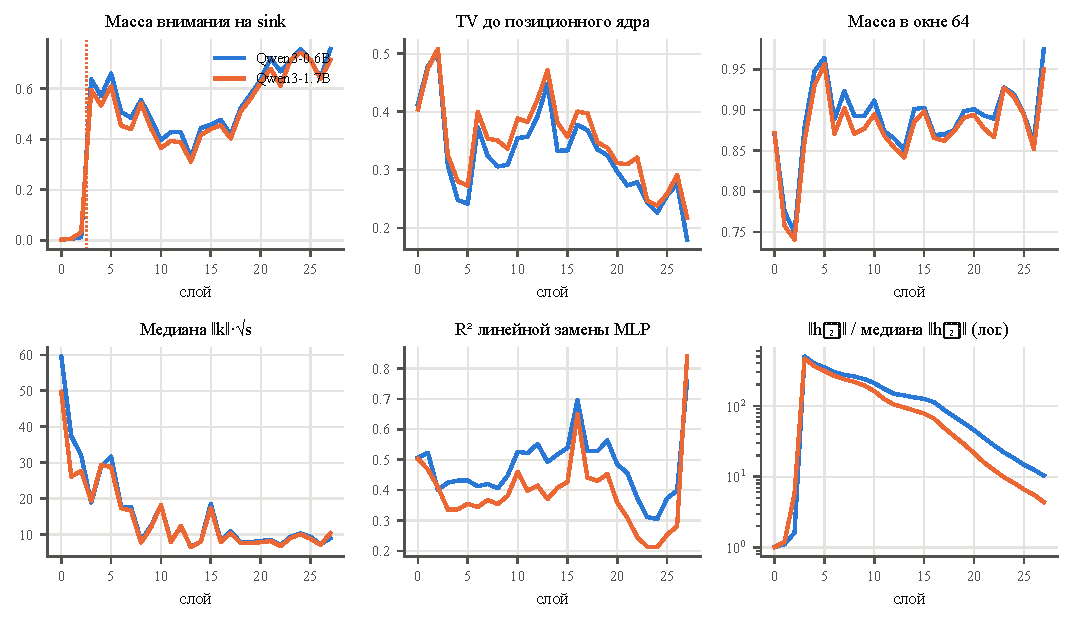
\includegraphics[width=\linewidth]{figures/profile.pdf}}
\caption{Послойный профиль Qwen3. Масса внимания на стоке (позиция 0);
расстояние полной вариации до позиционного ядра (меньше "--- позиционнее);
доля массы внимания в окне 64; медианная масштабированная норма ключей;
$R^2$ линейной замены MLP на отложенных данных; отношение нормы первого
токена к медиане остальных. Пунктир "--- $k_{\mathrm{sink}}$.}
\label{fig:profile}
\end{figure}

На Qwen3-0.6B первые три слоя образуют отдельный режим (рис.~\ref{fig:profile}).
В слоях 0--2 сток внимания практически отсутствует: доля массы на
позиции 0 составляет $0.3$--$1.3\%$ против $32$--$77\%$ в последующих
слоях. Норма состояния первого токена выросла с ${\approx}20$ до
${\approx}7000$ к моменту входа в слой~3. Поэтому $k_{\mathrm{sink}}=3$.
Вопреки исходной гипотезе о <<позиционных>> первых слоях, расстояние
до позиционного ядра в слоях 0--2 наибольшее
($\mathrm{TV}\approx0.42$--$0.50$ против $0.30$ в среднем по слоям 3--27,
разброс $0.17$--$0.44$): внимание
первых слоёв в основном контентное. Это мотивирует метод O4.
На Qwen3-1.7B картина та же: $k_{\mathrm{sink}}=3$, норма первого
токена достигает ${\approx}14\,700$ на входе слоя~3.

\subsection{Случайные признаки неприменимы к первым слоям}

\begin{figure}[t]
\centering
\figorpending{figures/favor.pdf}{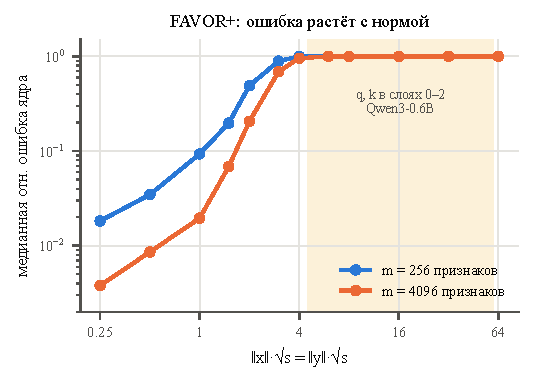
\includegraphics[width=0.55\linewidth]{figures/favor.pdf}}
\caption{Медианная относительная ошибка оценки $\exp(x^\top y)$
признаками FAVOR+ в зависимости от нормы входа ($D=128$, 64 пары на
точку, ошибка ограничена сверху единицей). Закрашенная
область "--- нормы запросов и ключей в слоях 0--2 Qwen3-0.6B.}
\label{fig:favor}
\end{figure}

Дисперсия оценки FAVOR+ растёт как $\exp(\|x+y\|^2)$. Для $m=4096$
признаков медианная относительная ошибка равна $2\%$ при
$\|x\|\sqrt s=\|y\|\sqrt s=1$, $21\%$ при $2$, $69\%$ при $3$ и
${\approx}100\%$ начиная с $4$. У Qwen3-0.6B после QK-нормализации медианная
масштабированная норма ключей в слоях 0--2 равна $32$--$60$, запросов
"--- $4.5$--$8$ (рис.~\ref{fig:favor}). Оценка ядра в этой области
бессмысленна, и замена внимания Performer без переобучения разрушает
модель. Мы проверили, что реализация несмещённая при малых нормах, то
есть это свойство модели, а не ошибка кода.

\subsection{Зависимость от глубины замены}

\begin{figure}[t]
\centering
\figorpending{figures/howmany.pdf}{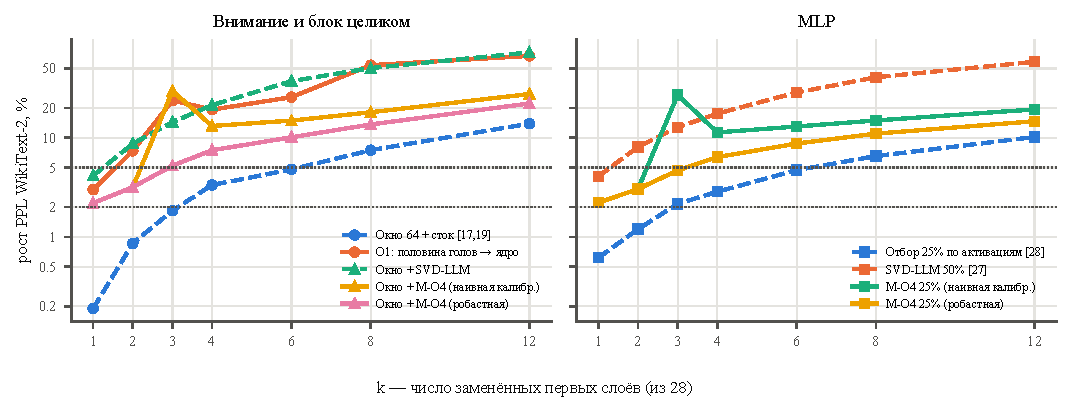
\includegraphics[width=\linewidth]{figures/howmany.pdf}}
\caption{Рост PPL WikiText-2 в зависимости от числа заменённых первых
слоёв $k$ (Qwen3-0.6B, 32 окна по 1024 токена, логарифмическая шкала;
пунктирные линии "--- пороги 2 и 5\,\%). Пунктир с кружками "--- методы из
литературы, сплошные с квадратами "--- предложенные; для M-O4 показаны
наивная и робастная калибровка (разд.~\ref{sec:propagation}).}
\label{fig:howmany}
\end{figure}

Окно со стоком деградирует плавно: 0.2, 0.9, 1.8, 3.3, 4.8, 7.5 и
13.9\,\% при $k = 1, 2, 3, 4, 6, 8, 12$, то есть первые три слоя
внимания заменяются в пределах 2\,\%, первые шесть "--- в пределах 5\,\%,
и даже при замене почти половины слоёв потеря остаётся умеренной. Отбор
25\,\% нейронов по готовым активациям ведёт себя похоже (0.6 "--- 10.2\,\%),
но экономит лишь последнюю матрицу MLP. SVD-LLM и O1 разваливаются
быстро: 12.8 и 23.7\,\% уже при $k=3$, более 50\,\% при $k=8$. Наивно
откалиброванный M-O4 демонстрирует немонотонность с пиком при
$k = k_{\mathrm{sink}} = 3$; её причина и устранение "--- в
разд.~\ref{sec:propagation}, после чего M-O4 удерживает 5\,\% до $k=3$ и
остаётся лучшим из методов с предсказанием нейронов до их вычисления.

\subsection{Качество и бюджет вычислений}

\begin{figure}[t]
\centering
\figorpending{figures/pareto.pdf}{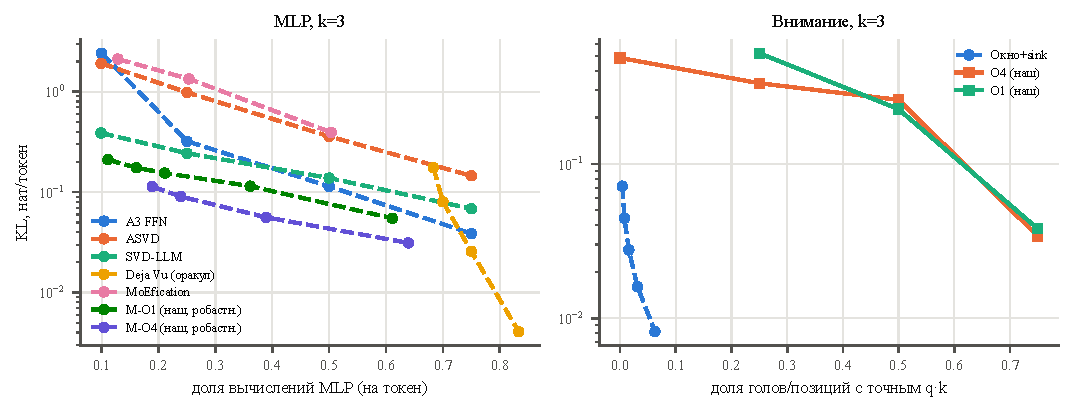
\includegraphics[width=\linewidth]{figures/pareto.pdf}}
\caption{KL в зависимости от бюджета при $k=k_{\mathrm{sink}}$ (Qwen3-0.6B).
Слева "--- методы для MLP (доля умножений на токен относительно
исходного MLP), справа "--- методы для внимания (доля вычисляемых
$q^\top k$).}
\label{fig:pareto}
\end{figure}

Ширина окна при $k=3$ задаёт плавный компромисс: 8, 16, 32, 64 и 128
позиций дают рост PPL 6.3, 4.1, 2.9, 1.8 и 1.0\,\%, то есть каждое
удвоение окна снимает около трети ошибки; 64 "--- колено кривой, которое мы
и используем. Для MLP отбор по вкладу нейрона при 5, 10, 25 и 50\,\%
активных даёт 16.9, 6.8, 2.2 и 0.3\,\%; робастный M-O4 с предсказанием
нейронов "--- 10.2, 7.8, 4.7 и 2.5\,\% при стоимости $0.28$--$0.55$ MLP;
SVD-LLM при ранге 10--75\,\% "--- от 41.5 до 5.8\,\%; A3 FFN "--- от $10^3$\,\%
при 10\,\% нейронов до 3.1\,\% при 75\,\%; ASVD и MoEfication уступают
всем. Для внимания половина голов, заменённых позиционным ядром (O1),
стоит 23.7\,\%, четверть "--- 2.9\,\%, три четверти "--- 67\,\%: позиционными
являются лишь немногие головы первых слоёв.

\subsection{Единый обменный курс}

\begin{figure}[t]
\centering
\figorpending{figures/exchange.pdf}{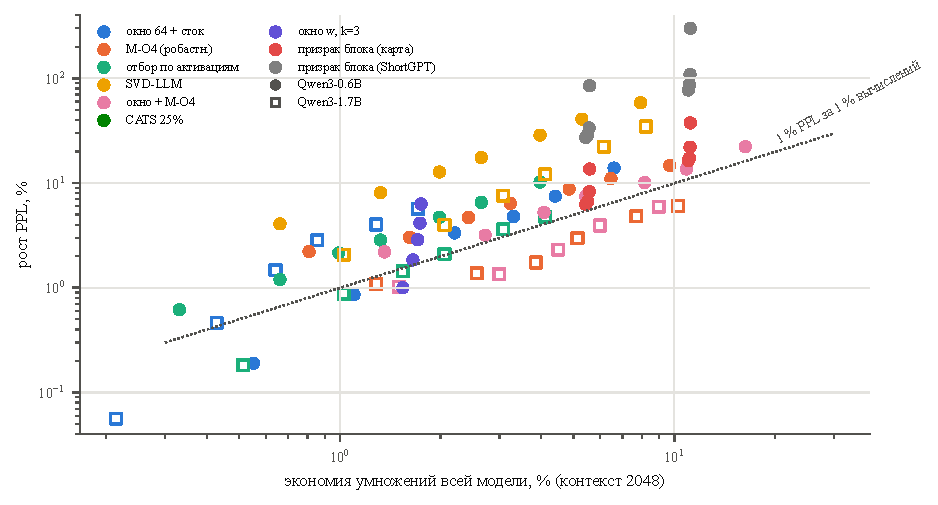
\includegraphics[width=0.9\linewidth]{figures/exchange.pdf}}
\caption{Все замены на одной шкале: рост PPL против доли сэкономленных
умножений всей модели при контексте 2048 (кривые по $k$, ширина окна,
призраки блоков; закрашенные маркеры "--- Qwen3-0.6B, пустые "--- 1.7B).
Пунктир "--- один процент PPL за один процент вычислений.}
\label{fig:exchange}
\end{figure}

На рис.~\ref{fig:exchange} все работающие детерминированные замены
Qwen3-0.6B ложатся около линии <<один процент PPL за один процент
вычислений>>: окно при $k=3$ (1.7\,\% экономии за 1.8\,\%), робастный M-O4
при $k=3$ ($\approx 4.6$ за 4.7\,\%), линейный призрак двух средних слоёв
(6.5 за 6.2\,\%). Методы с ошибочным критерием "--- SVD-LLM, CATS, призраки
по косинусному критерию ShortGPT "--- лежат в разы выше. У Qwen3-1.7B курс
лучше примерно в 2.5 раза: те же замены стоят 0.4\,\% PPL за процент
вычислений. Это основной аргумент в пользу проверки на моделях 4B--32B:
если курс продолжает улучшаться с размером, замена первых слоёв
становится выгодной именно там, где важна.

\subsection{Призраки блоков: где удалять слои}

Линейная замена блока из $n$ подряд идущих слоёв
(ReplaceMe~\cite{shopkhoev2025replaceme}) требует выбрать блок.
Критерий ShortGPT "--- косинусная близость входа и выхода слоя "--- на
Qwen3-0.6B выбирает слои 24--25 и 23--26; их удаление стоит $+85$ и
$+1760\,\%$ PPL, а линейная карта на границе снижает это лишь до 27 и
77\,\%. Выбор по нашей карте (минимальный KL одиночного удаления) даёт
слои 13--14 и 12--15: удаление $+13.6$ и $+37.5\,\%$, с полной линейной
картой $6.2$ и $16.4\,\%$, с картой ранга 256 "--- $6.7$ и $17.3\,\%$. Карта
заменяемости, построенная за один прогон одиночных замен, выбирает блок
в 4--5 раз точнее косинусного критерия, а призрак двух средних слоёв по
цене сопоставим с заменой MLP трёх первых.

\subsection{Итоговая таблица}

\begin{table}[t]
\centering
\scriptsize
\setlength{\tabcolsep}{3pt}
\IfFileExists{tables/final_0.6b.tex}{\begin{tabular}{lrrrrrrrrrrr}
\toprule
 & Исх. & Окно & Окно$_m$ & Поз. & A3 & SVD-LLM & Окно+SVD & O1 & M-O4 & M-O4r & Окно+M-O4r \\
\midrule
Что заменено & — & вним. & вним. & вним. & блок & MLP & блок & вним. & MLP & MLP & блок \\
Доля вычислений MLP & 1.00 & 1.00 & 1.00 & 1.00 & 0.50 & 0.50 & 0.50 & 1.00 & 0.39 & 0.39 & 0.39 \\
PPL WikiText-2 $\downarrow$ & 14.06 & 14.32 & 14.32 & 84.26 & 20.98 & 15.85 & 16.08 & 17.39 & 17.86 & 14.72 & 14.79 \\
KL к исходной $\downarrow$ & 0.000 & 0.016 & 0.016 & 1.805 & 0.433 & 0.138 & 0.151 & 0.226 & 0.268 & 0.056 & 0.065 \\
Совпадение top-1 $\uparrow$ & 100.0 & 94.7 & 94.7 & 43.4 & 71.6 & 85.4 & 84.3 & 80.3 & 76.1 & 90.5 & 89.4 \\
LAMBADA $\uparrow$ & 53.5 & 55.0 & 55.0 & 14.5 & 36.5 & 46.0 & 46.0 & — & 32.5 & 51.0 & 51.5 \\
HellaSwag $\uparrow$ & 53.0 & 53.5 & 53.5 & 47.0 & 47.5 & 53.0 & 53.0 & — & 48.5 & 54.0 & 53.0 \\
ARC-e $\uparrow$ & 55.5 & 57.5 & 57.5 & 49.5 & 54.0 & 61.0 & 61.0 & — & 57.0 & 58.0 & 57.0 \\
ARC-c $\uparrow$ & 36.0 & 37.0 & 37.0 & 28.5 & 30.0 & 35.0 & 35.0 & — & 31.0 & 37.0 & 38.0 \\
PIQA $\uparrow$ & 72.0 & 70.5 & 70.5 & 61.0 & 64.5 & 67.5 & 68.0 & — & 64.0 & 69.0 & 68.0 \\
WinoGrande $\uparrow$ & 63.0 & 63.0 & 63.0 & 58.0 & 57.0 & 59.0 & 59.5 & — & 53.5 & 64.5 & 65.5 \\
MMLU (5-shot) $\uparrow$ & 51.6 & 50.9 & 51.6 & 29.1 & 37.2 & 48.8 & 46.0 & — & 24.6 & 48.8 & 47.0 \\
Среднее по бенчам $\uparrow$ & 54.9 & 55.3 & 55.4 & 41.1 & 46.7 & 52.9 & 52.6 & — & 44.4 & 54.6 & 54.3 \\
\bottomrule
\end{tabular}
}{\textcolor{red}{[ожидает прогона]}}
\caption{Qwen3-0.6B-Base, замена первых $k_{\mathrm{sink}}$ слоёв.
Столбцы: исходная модель; методы из литературы (окно+сток, позиционное
внимание, A3, SVD-LLM, окно+SVD-LLM); предложенные (O1, M-O4 с наивной
и робастной калибровкой, окно+M-O4 робастный). Бенчмарки "--- точность,
\%, подвыборки по 200 примеров (MMLU "--- 5 на подзадачу).}
\label{tab:final06}
\end{table}

\begin{table}[t]
\centering
\scriptsize
\setlength{\tabcolsep}{3pt}
\IfFileExists{tables/final_1.7b.tex}{\begin{tabular}{lrrrrrrrrrrr}
\toprule
 & Исх. & Окно & Окно$_m$ & Поз. & A3 & SVD-LLM & Окно+SVD & O1 & M-O4 & M-O4r & Окно+M-O4r \\
\midrule
Что заменено & — & вним. & вним. & вним. & блок & MLP & блок & вним. & MLP & MLP & блок \\
Доля вычислений MLP & 1.00 & 1.00 & 1.00 & 1.00 & 0.50 & 0.50 & 0.50 & 1.00 & 0.38 & 0.38 & 0.38 \\
PPL WikiText-2 $\downarrow$ & 10.39 & 10.54 & 10.54 & 22.07 & 15.06 & 11.18 & 11.33 & 11.36 & 10.60 & 10.57 & 10.63 \\
KL к исходной $\downarrow$ & 0.000 & 0.019 & 0.019 & 0.781 & 0.408 & 0.091 & 0.104 & 0.088 & 0.031 & 0.028 & 0.037 \\
Совпадение top-1 $\uparrow$ & 100.0 & 94.3 & 94.4 & 62.5 & 73.9 & 88.8 & 87.5 & 87.9 & 93.5 & 94.0 & 92.4 \\
LAMBADA $\uparrow$ & 64.0 & 63.5 & 64.0 & 36.0 & 51.0 & 60.5 & 61.0 & 60.5 & 64.5 & 64.0 & 65.5 \\
HellaSwag $\uparrow$ & 57.0 & 59.5 & 59.5 & 55.0 & 55.5 & 58.0 & 57.5 & 57.5 & 56.5 & 59.5 & 60.0 \\
ARC-e $\uparrow$ & 68.0 & 69.0 & 69.0 & 69.5 & 59.5 & 71.5 & 72.0 & 74.0 & 70.5 & 70.5 & 72.0 \\
ARC-c $\uparrow$ & 43.5 & 43.5 & 43.5 & 43.0 & 38.0 & 47.0 & 46.5 & 45.5 & 46.0 & 43.5 & 44.5 \\
PIQA $\uparrow$ & 77.5 & 79.0 & 79.0 & 75.5 & 69.5 & 72.5 & 72.0 & 75.5 & 73.0 & 77.0 & 76.0 \\
WinoGrande $\uparrow$ & 61.5 & 61.0 & 61.0 & 56.0 & 55.5 & 62.5 & 63.0 & 60.0 & 65.0 & 64.0 & 65.0 \\
MMLU (5-shot) $\uparrow$ & 64.6 & 65.6 & 67.7 & 37.2 & 45.6 & 58.9 & 58.2 & 64.9 & 63.5 & 66.3 & 64.2 \\
Среднее по бенчам $\uparrow$ & 62.3 & 63.0 & 63.4 & 53.2 & 53.5 & 61.6 & 61.5 & 62.6 & 62.7 & 63.5 & 63.9 \\
\bottomrule
\end{tabular}
}{\textcolor{red}{[ожидает прогона]}}
\caption{Qwen3-1.7B-Base, те же столбцы, что в табл.~\ref{tab:final06}.}
\label{tab:final17}
\end{table}

\paragraph{Статистическая значимость.} На подвыборках по 200 примеров
стандартная ошибка средней точности по семи задачам равна $\pm2.5$ п.п.,
на 1000 примерах "--- $\pm1.1$ п.п. (биномиальная оценка). На 1000 примерах
окно при $k=3$ даёт 54.7 против 54.5\,\% у исходной Qwen3-0.6B и 62.9
против 62.4\,\% у 1.7B "--- неотличимо от исходной модели. Робастный M-O4
на 0.6B теряет около пункта (53.5\,\%, на границе значимости), на 1.7B
"--- нет (62.7\,\%); SVD-LLM теряет один--два пункта значимо (52.5 и
61.5\,\%). Для PPL и KL 95\,\%-е интервалы по бутстрэпу окон на полном
тесте WikiText-2 узки: окно 1.6 [1.5; 1.7]\,\%, робастный M-O4 4.9
[4.6; 5.1]\,\%, SVD-LLM 13.2 [12.6; 13.8]\,\% на 0.6B; 1.7 [1.6; 1.8], 1.7
[1.5; 1.9] и 8.2 [7.7; 8.7]\,\% на 1.7B (табл.~\ref{tab:ci}). Все
различия между главными столбцами значимы.

\begin{table}[t]
\centering
\scriptsize
\IfFileExists{tables/ci_0.6b.tex}{\begin{tabular}{lllll}
\toprule
Конфигурация & рост PPL, \% [95\% ДИ] & KL [95\% ДИ] & среднее по бенчам ± 1.96 SE & источник \\
\midrule
orig & 0.0 [0.0; 0.0] & 0.000 [0.000; 0.000] & 54.5 ± 1.1 & ci+bench1000 \\
L1-window64 & 1.6 [1.5; 1.7] & 0.015 [0.015; 0.015] & 54.7 ± 1.1 & ci+bench1000 \\
MO4-routed25r & 4.9 [4.6; 5.1] & 0.059 [0.057; 0.061] & 53.5 ± 1.1 & ci+bench1000 \\
ML5-svdllm50 & 13.2 [12.6; 13.8] & 0.145 [0.140; 0.151] & 52.5 ± 1.1 & ci+bench1000 \\
B-window+MO4-25r & 5.4 [5.1; 5.7] & 0.067 [0.065; 0.070] & 53.5 ± 1.1 & ci+bench1000 \\
\bottomrule
\end{tabular}
}{\textcolor{red}{[ожидает прогона]}}
\caption{Qwen3-0.6B, $k=3$: рост PPL и KL на полном тесте WikiText-2 с
95\,\%-ми интервалами по бутстрэпу окон (283 окна по 1024 токена).}
\label{tab:ci}
\end{table}

\subsection{Длина контекста и число стоков}

Ошибка окна растёт с длиной контекста медленно, примерно как логарифм
$T$: при $k=3$ она равна 1.81, 2.51, 3.21 и 4.89\,\% для $T = 1024$, 2048,
4096 и 8192 (табл.~\ref{tab:long}); четыре стока вместо одного помогают
лишь при $T=8192$ (4.49\,\%). Число стоков "--- один, два, четыре или сток
вместе со всеми токенами перевода строки "--- на результат не влияет
(разброс 0.03 п.п. при $k=3$ и $k=6$).

\begin{table}[t]
\centering
\small
\IfFileExists{tables/long.tex}{\begin{tabular}{lrrrr}
\toprule
Контекст $T$ & 1024 & 2048 & 4096 & 8192 \\
\midrule
$k=3$, 1 сток & 1.81\% & 2.51\% & 3.21\% & 4.89\% \\
$k=3$, 4 стока & 1.80\% & 2.48\% & 3.18\% & 4.49\% \\
\midrule
$k=3$, 2 стока & 1.81\% & 2.49\% & — & — \\
$k=3$, сток + переводы строки & 1.80\% & 2.49\% & — & — \\
$k=6$, 2 стока & 4.69\% & 6.27\% & — & — \\
$k=6$, сток + переводы строки & 4.71\% & 6.28\% & — & — \\
\bottomrule
\end{tabular}
}{\textcolor{red}{[ожидает прогона]}}
\caption{Окно 64 в первых $k$ слоях Qwen3-0.6B: рост PPL в зависимости
от длины контекста и числа стоков (бюджет 65 тыс. токенов на длину).}
\label{tab:long}
\end{table}

\subsection{Перенос на другой корпус}

\begin{figure}[t]
\centering
\figorpending{figures/domain.pdf}{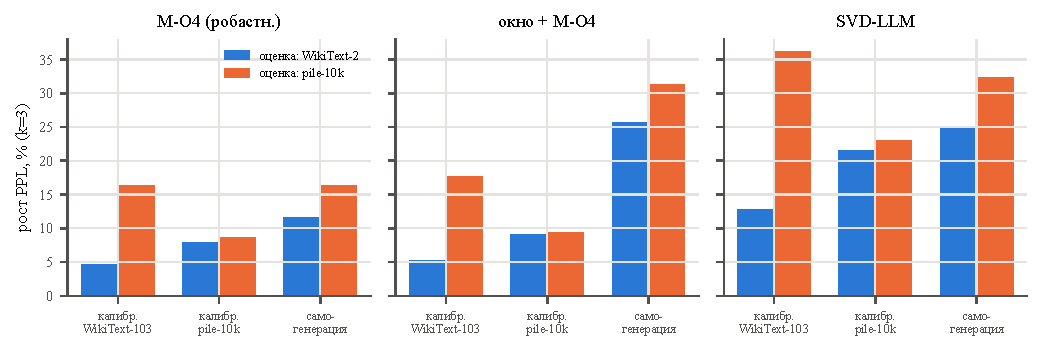
\includegraphics[width=\linewidth]{figures/domain.pdf}}
\caption{Домен калибровки (Qwen3-0.6B, $k=3$): рост PPL на WikiText-2 и
на pile-10k при калибровке на WikiText-103, на pile-10k и на тексте,
сгенерированном самой моделью.}
\label{fig:domain}
\end{figure}

Окно не калибруется и переносится без потерь: 1.2\,\% на pile-10k против
1.8\,\% на WikiText-2. Калиброванные замены MLP переобучаются под домен
калибровки: при калибровке на WikiText-103 робастный M-O4 стоит 4.7\,\% на
WikiText-2 и 16.4\,\% на pile-10k, SVD-LLM "--- 12.8 и 36\,\%
(рис.~\ref{fig:domain}). Калибровка на pile-10k выравнивает ошибку
(8.6 и 8.0\,\% у M-O4, 23 и 21.5\,\% у SVD-LLM), то есть смешанная
калибровка "--- рабочее лекарство; текст, сгенерированный самой моделью,
лекарством не является (16.3 и 11.6\,\%): сэмплы нерепрезентативны.

\subsection{Второе семейство: SmolLM2-1.7B и Llama-3.2-1B}
\label{sec:family2}

Таблицы~\ref{tab:finalsmol} и~\ref{tab:finalllama} повторяют итоговую
таблицу для двух моделей архитектуры Llama. Глубина $k_{\mathrm{sink}}$
определяется профилем автоматически: у Llama-3.2-1B массивная активация
позиции~0 (норма 794 при медиане 2.4) появляется после слоя~1, как у
Qwen3 "--- после слоя~2, поэтому $k_{\mathrm{sink}}=2$; у SmolLM2 сток
позиции~0 (норма $26\,235$) возникает лишь после слоя~7, $k_{\mathrm{sink}}=8$.
Три вывода. (1) Правило стока в исходном виде (<<позиция~0>>) для этого
семейства неверно: окно 64 с одним стоком даёт $+64\,\%$ PPL на SmolLM2
при $k=8$ и $+13\,\%$ на Llama-3.2-1B при $k=2$, тогда как то же окно с
правилом <<сток "--- массивный ключ>> (разд.~\ref{sec:tokensinks}) "---
$4.4$ и $2.8\,\%$, то есть столько же слоёв, сколько у Qwen3 при пороге
5\,\%. На кривой по $k$ у SmolLM2 окно с позиционным стоком стоит 0.7, 2.1,
13.7, 27.3, 62.4 и 64.1\,\% при $k=1,2,3,4,6,8$; с массивными стоками "---
0.8, 1.8, 2.0, 2.2, 3.5 и 4.4\,\% при тех же $k$, то есть та же форма кривой,
что у Qwen3. (2) MLP первых слоёв у
Llama-семейства заменяется заметно хуже, чем у Qwen3: робастный M-O4 стоит
$16\,\%$ на Llama-3.2-1B уже при $k=2$ и $6.3\,\%$ на SmolLM2 при $k=1$
(34\,\% при $k=8$), SVD-LLM "--- 47 и 49\,\%, A3 "--- 97 и 499\,\%,
позиционное внимание (relpos) и типизация голов O1 рушатся при $k\ge2$.
Диагностика обрыва показывает, что усиление ошибки по слоям $k-1..k+1$ у
SmolLM2 равно 0.9--1.1, то есть обрыва нет: дорог сам первый MLP, а не
его последствия для стока. Оракульный отбор 25\,\% нейронов одного слоя~0
даёт KL 0.0046 (меньше, чем у Qwen3-0.6B), так что узкое место "---
линейный предиктор нейронов при $I/d=4$, а не отбор как таковой.
(3) Робастная калибровка и защита нейронов стока нужны здесь ещё
сильнее: наивная комбинация окно\,+\,M-O4 даёт $+1\,100\,\%$ на
Llama-3.2-1B и $+612\,\%$ на SmolLM2 ($k=2$), робастная с защитой "---
31.8 и 13.9\,\%; наивный M-O4 на SmolLM2 при $k=2$ стоит 123\,\%, с защитой
нейронов стока "--- 11.3\,\%. Бенчмарки в таблицах посчитаны на тех же
подвыборках, что и для Qwen3.

\begin{table}[t]
\centering
\scriptsize
\setlength{\tabcolsep}{3pt}
\IfFileExists{tables/final_smol1.7b.tex}{\begin{tabular}{lrrrrrrrrrrr}
\toprule
 & Исх. & Окно & Окно$_m$ & Поз. & A3 & SVD-LLM & Окно+SVD & O1 & M-O4 & M-O4r & Окно+M-O4r \\
\midrule
Что заменено & — & вним. & вним. & вним. & блок & MLP & блок & вним. & MLP & MLP & блок \\
Доля вычислений MLP & 1.00 & 1.00 & 1.00 & — & 0.50 & — & — & — & 0.35 & 0.35 & 0.35 \\
PPL WikiText-2 $\downarrow$ & 8.93 & 14.65 & 9.32 & — & 53.47 & — & — & — & 12.00 & 12.00 & 17.74 \\
KL к исходной $\downarrow$ & 0.000 & 0.503 & 0.044 & — & 1.795 & — & — & — & 0.314 & 0.313 & 0.713 \\
Совпадение top-1 $\uparrow$ & 100.0 & 79.3 & 91.2 & — & 48.4 & — & — & — & 77.6 & 77.7 & 65.7 \\
LAMBADA $\uparrow$ & 71.0 & 66.5 & 71.5 & — & 27.5 & — & — & — & 34.0 & 35.0 & 16.5 \\
HellaSwag $\uparrow$ & 64.0 & 63.5 & 63.5 & — & 41.0 & — & — & — & 52.5 & 52.0 & 46.0 \\
ARC-e $\uparrow$ & 75.0 & 75.5 & 75.5 & — & 32.5 & — & — & — & 57.5 & 56.0 & 43.0 \\
ARC-c $\uparrow$ & 43.0 & 43.5 & 43.5 & — & 19.0 & — & — & — & 29.0 & 30.0 & 25.0 \\
PIQA $\uparrow$ & 78.0 & 78.0 & 78.5 & — & 51.0 & — & — & — & 62.0 & 63.0 & 58.5 \\
WinoGrande $\uparrow$ & 65.0 & 66.0 & 66.0 & — & 46.5 & — & — & — & 58.0 & 59.5 & 57.0 \\
MMLU (5-shot) $\uparrow$ & 56.1 & 54.0 & 53.0 & — & 22.5 & — & — & — & 28.1 & 29.5 & 21.4 \\
Среднее по бенчам $\uparrow$ & 64.6 & 63.9 & 64.5 & — & 34.3 & — & — & — & 45.9 & 46.4 & 38.2 \\
\bottomrule
\end{tabular}
}{\textcolor{red}{[ожидает прогона]}}
\caption{SmolLM2-1.7B, замена первых $k_{\mathrm{sink}}=8$ слоёв; столбцы
как в табл.~\ref{tab:final06} (конфигурации, не поместившиеся в память
ноутбука при $k=8$, опущены). Окно с массивными стоками (L1-window64s) "---
правило разд.~\ref{sec:tokensinks}.}
\label{tab:finalsmol}
\end{table}

\begin{table}[t]
\centering
\scriptsize
\setlength{\tabcolsep}{3pt}
\IfFileExists{tables/final_llama1b.tex}{\begin{tabular}{lrrrrrrrrrrr}
\toprule
 & Исх. & Окно & Окно$_m$ & Поз. & A3 & SVD-LLM & Окно+SVD & O1 & M-O4 & M-O4r & Окно+M-O4r \\
\midrule
Что заменено & — & вним. & вним. & вним. & блок & MLP & блок & вним. & MLP & MLP & блок \\
Доля вычислений MLP & 1.00 & 1.00 & 1.00 & 1.00 & 0.50 & 0.50 & 0.50 & 1.00 & 0.35 & 0.35 & 0.35 \\
PPL WikiText-2 $\downarrow$ & 11.31 & 12.80 & 11.62 & 8803.33 & 22.23 & 16.58 & 20.87 & 14.75 & 13.14 & 13.14 & 14.90 \\
KL к исходной $\downarrow$ & 0.000 & 0.113 & 0.030 & 6.630 & 0.665 & 0.384 & 0.602 & 0.258 & 0.151 & 0.152 & 0.280 \\
Совпадение top-1 $\uparrow$ & 100.0 & 86.2 & 92.5 & 1.0 & 65.4 & 74.1 & 67.8 & 78.5 & 84.2 & 84.1 & 77.9 \\
LAMBADA $\uparrow$ & 59.0 & 59.0 & 59.0 & 0.0 & 44.5 & 45.0 & 45.5 & 59.5 & 55.5 & 54.0 & 50.5 \\
HellaSwag $\uparrow$ & 58.0 & 59.0 & 59.0 & 31.5 & 55.5 & 57.5 & 57.5 & 57.5 & 57.0 & 55.5 & 54.5 \\
ARC-e $\uparrow$ & 60.5 & 61.0 & 61.0 & 26.0 & 50.0 & 52.5 & 53.0 & 61.0 & 58.5 & 58.0 & 55.5 \\
ARC-c $\uparrow$ & 32.5 & 32.5 & 32.5 & 27.0 & 27.5 & 28.5 & 28.0 & 33.5 & 32.5 & 32.0 & 34.0 \\
PIQA $\uparrow$ & 76.5 & 75.5 & 75.5 & 46.5 & 67.0 & 71.5 & 72.5 & 75.5 & 70.0 & 70.0 & 69.0 \\
WinoGrande $\uparrow$ & 62.5 & 63.5 & 63.5 & 51.0 & 54.5 & 58.0 & 57.0 & 59.0 & 63.5 & 59.5 & 59.0 \\
MMLU (5-shot) $\uparrow$ & 35.1 & 32.6 & 32.6 & 27.0 & 26.3 & 26.0 & 28.8 & 28.8 & 32.3 & 29.1 & 28.8 \\
Среднее по бенчам $\uparrow$ & 54.9 & 54.7 & 54.7 & 29.9 & 46.5 & 48.4 & 48.9 & 53.5 & 52.8 & 51.2 & 50.2 \\
\bottomrule
\end{tabular}
}{\textcolor{red}{[ожидает прогона]}}
\caption{Llama-3.2-1B, замена первых $k_{\mathrm{sink}}=2$ слоёв; столбцы
как в табл.~\ref{tab:final06}.}
\label{tab:finalllama}
\end{table}

\subsection{Время}

\begin{table}[t]
\centering
\scriptsize
\setlength{\tabcolsep}{4pt}
\IfFileExists{tables/timing.tex}{\begin{tabular}{lrrrrrr}
\toprule
Модель & $T$ & \multicolumn{2}{c}{слой внимания, мс} & \multicolumn{2}{c}{prefill модели, мс} & отношение \\
 & & полное (SDPA) & лента (PyTorch) & исходная & первые 3 слоя --- лента & \\
\midrule
Qwen3-0.6B & 1024 & 2.3 & 99.1 & 950 & 1275 & 0.74 \\
Qwen3-0.6B & 2048 & 8.5 & 209.3 & 2009 & 2657 & 0.76 \\
Qwen3-0.6B & 4096 & 37.6 & 457.7 & 4547 & 5695 & 0.80 \\
Qwen3-0.6B & 8192 & 163.2 & 894.5 & 11058 & 13331 & 0.83 \\
Qwen3-1.7B & 1024 & 2.2 & 96.9 & 2205 & 2557 & 0.86 \\
Qwen3-1.7B & 2048 & 7.6 & 193.6 & 4691 & 5287 & 0.89 \\
Qwen3-1.7B & 4096 & 29.7 & 386.7 & 9550 & 10696 & 0.89 \\
Qwen3-1.7B & 8192 & 155.7 & 808.6 & 21185 & 23572 & 0.90 \\
\bottomrule
\end{tabular}
}{\textcolor{red}{[ожидает прогона]}}
\caption{Замер времени на Apple M4 (MPS, bf16, медиана 5 запусков):
ленточная реализация окна на чистом PyTorch против fused-ядра SDPA.}
\label{tab:timing}
\end{table}

Наша ленточная реализация окна на чистом PyTorch, хотя и имеет
асимптотику $O(Tw)$ и память $O(Tw)$, на MPS медленнее fused-ядра
полного внимания в 5--40 раз на уровне слоя и замедляет prefill модели
на 10--25\,\% (табл.~\ref{tab:timing}). Реальное ускорение возможно только
со специализированным ядром скользящего окна, которые существуют для
CUDA; все оценки экономии в работе "--- по числу умножений.

\section{Распространение ошибки и робастная калибровка}\label{sec:propagation}

\subsection{Аномалия: обрыв на $k=3$}

Кривые на рис.~\ref{fig:howmany} для M-O4 и его комбинаций немонотонны:
при $k=2$ рост PPL составляет 3.0\,\%, при $k=3$ "--- 27.0\,\%, а при $k=4$
"--- снова 11.3\,\%. У окна, SVD-LLM и отбора нейронов по готовым
активациям кривые гладкие. Поскольку $k=3$ совпадает с
$k_{\mathrm{sink}}$ (разд.~\ref{sec:results}), первая гипотеза
естественна: слой~3, в котором впервые возникает сток внимания,
усиливает ошибку, пришедшую из заменённых слоёв, а при $k=4$ его
собственная калибровка её компенсирует. Послойная диагностика
(рис.~\ref{fig:cliff}) эту гипотезу опровергает и указывает на другой
механизм.

\begin{figure}[t]
\centering
\figorpending{figures/cliff.pdf}{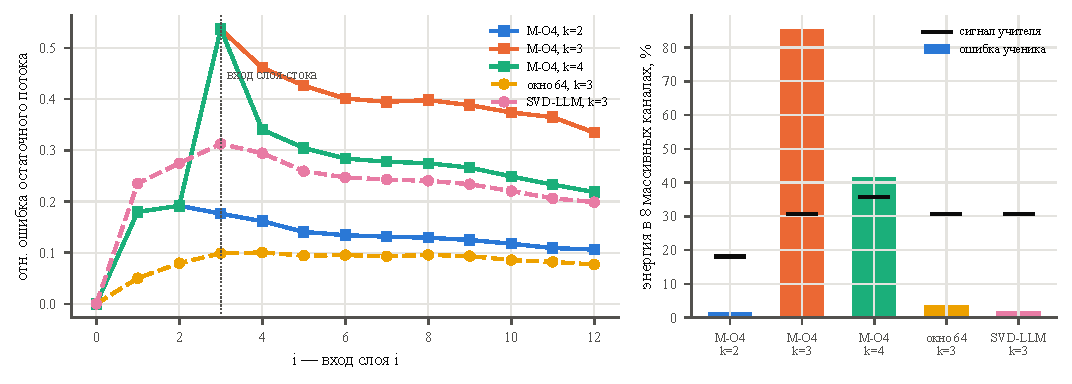
\includegraphics[width=\linewidth]{figures/cliff.pdf}}
\caption{Диагностика обрыва (Qwen3-0.6B, 8 окон по 1024 токена, позиции
$\ge 1$). Слева "--- относительная ошибка остаточного потока ученика на
входе каждого слоя. Справа "--- доля энергии ошибки на входе первого
незаменённого слоя, приходящаяся на 8 каналов массивной активации
(чёрточка "--- доля энергии сигнала учителя в тех же каналах).}
\label{fig:cliff}
\end{figure}

\subsection{Послойная диагностика}

Для каждой конфигурации мы сравниваем остаточный поток ученика и
учителя на входе каждого слоя (относительная ошибка по токенам, без
позиции~0). При $k=2$ ошибка после заменённых слоёв равна 0.18--0.19 и
далее монотонно убывает: каждый следующий слой гасит её с коэффициентом
около 0.9. При $k=3$ ошибка на входе слоя~3 равна 0.54, то есть скачок
происходит \emph{внутри заменённого слоя~2} (усиление 2.8), а слой~3
её не усиливает (коэффициент 0.86). Ошибка структурирована: 85\,\% её
энергии приходится на 8 каналов массивной активации, тогда как у
сигнала учителя в этих каналах 31\,\% энергии, у окна "--- 3.6\,\%, у
SVD-LLM "--- 1.7\,\%. Это сдвигает масштаб токенов именно в тех
координатах, по которым слой~3 отличает сток от остальных токенов:
средняя масса внимания на позиции~0 падает с 0.63 до 0.50, а средняя
абсолютная разность по позициям составляет 0.15. При $k=4$ калибровка
слоя~3 с компенсацией дрейфа снижает ошибку с 0.54 до 0.34, что и даёт
«восстановление» на кривой.

\subsection{Причина: одна строка калибровочной выборки}

MLP слоя~2 "--- тот блок, который создаёт массивную активацию: норма
остаточного потока на позиции~0 растёт с 19 до $\approx 7\,000$ именно
на его выходе. Калибровочная выборка состоит из 256 окон по 512
токенов, вырезанных из текста без начального токена. В $1.6\,\%$ таких
окон (33 из 2\,048 в большом пуле) модель образует сток не на позиции~0,
а на токене вроде <<0>>, <<8>> или <<=>> на позиции 1--2: выход MLP слоя~2
для него имеет норму $6\,400$--$7\,100$ при медиане $4.9$. В первых 32 тыс.
токенов нашей выборки такая строка одна и несёт $98.2\,\%$ энергии целей
$\sum_t\|y_t\|^2$; во всей выборке их около четырёх. Задача наименьших
квадратов для линейной поправки и предиктора нейронов M-O4 подгоняется
под эти строки, и ошибка в массивных каналах появляется у всех токенов.
Слои 0 и~1 не затронуты, потому что до слоя~2 массивной активации ещё
нет; в оценочных окнах таких токенов нет вовсе.

Ту же причину имеет неудача «корректоров»: поканальная, полная
($d\times d$), низкоранговая и ограниченная массивными каналами
линейные карты на входе слоя~3, подогнанные по сырым остаткам, не
уменьшают, а увеличивают рост PPL (с 27 до 35--45\,\%), поскольку те же
строки доминируют и в регрессорах.

\subsection{Формальная оценка: влияние одной строки}

Все рассматриваемые калибровки сводятся к гребневой регрессии
$W = (\Phi^\top\Phi + \lambda I)^{-1}\Phi^\top Y$ по строкам
$(\varphi_t, y_t)$, где $\varphi_t$ "--- признаки токена $t$ (вход блока с
единицей для смещения), $y_t$ "--- цель. Пусть строка $o$ добавлена к
набору $S$ остальных строк, $A = \Phi_S^\top\Phi_S + \lambda I$,
$W_S = A^{-1}\Phi_S^\top Y_S$ "--- решение без неё, $r_o = y_o -
\varphi_o^\top W_S$ "--- её невязка относительно этого решения и
$h_o = \varphi_o^\top A^{-1}\varphi_o$ "--- её рычаг.

\begin{proposition}\label{prop:leverage}
Решение с добавленной строкой равно
$W_{S\cup o} = W_S + \dfrac{A^{-1}\varphi_o\, r_o^\top}{1 + h_o}$, и для
любого токена $t$ изменение предсказания равно
\[
\Delta\hat y_t = \frac{c_{t}}{1 + h_o}\, r_o, \qquad c_t = \varphi_t^\top A^{-1}\varphi_o,
\]
так что $\|\Delta\hat y_t\| \le \dfrac{|c_t|}{1+h_o}\,\|r_o\|$, причём
$\Delta\hat y_t$ направлено вдоль $r_o$ для всех $t$ одновременно.
\end{proposition}

\begin{proof}
По формуле Шермана"--~Моррисона $(A + \varphi_o\varphi_o^\top)^{-1} =
A^{-1} - \frac{A^{-1}\varphi_o\varphi_o^\top A^{-1}}{1 + h_o}$. Подставляя в
$W_{S\cup o} = (A + \varphi_o\varphi_o^\top)^{-1}(\Phi_S^\top Y_S +
\varphi_o y_o^\top)$ и группируя слагаемые, получаем
$W_{S\cup o} - W_S = \frac{A^{-1}\varphi_o}{1+h_o}\,(y_o -
\varphi_o^\top W_S)^\top$; умножение слева на $\varphi_t^\top$ даёт
утверждение.
\end{proof}

Предложение объясняет два наблюдения и опровергает третье. Во-первых,
ошибка от строки с массивной активацией у \emph{всех} токенов лежит в
одном направлении $r_o$ "--- в каналах массивной активации (85\,\%
энергии ошибки на рис.~\ref{fig:cliff}). Во-вторых, её величина
пропорциональна $\|r_o\|$ и связи $c_t$. Измерения на слое~2
(табл.~\ref{tab:leverage}) подтверждают формулу: отклонение
$W_{S\cup o}-W_S$ от предсказания Шермана"--~Моррисона составляет
$4\cdot10^{-5}$, а предсказанная утечка в обычные токены "--- около половины
нормы их целей (медиана $53\,\%$ на 0.6B и $47\,\%$ на 1.7B). Третье
наблюдение "--- отсутствие обрыва на Qwen3-1.7B при том же выбросе
(норма $14\,355$) "--- предложение \emph{не} объясняет: утечка там такая же.
Разница в следующем слое: на 0.6B возмущение массивных каналов снижает
массу стока в слое~3 с $0.63$ до $0.50$, на 1.7B она не меняется
($0.589$ против $0.586$), и дальнейшие слои гасят ошибку. Иммунитет
большей модели "--- свойство устойчивости её стока, а не регрессии.
Величины $h_o$, $\|r_o\|$ и $\overline{|c_t|}$ измеримы \emph{до}
построения замены и дают априорный критерий опасности калибровочной
выборки.

\begin{table}[t]
\centering
\scriptsize
\setlength{\tabcolsep}{4pt}
\begin{tabular}{lrrrrrr}
\toprule
Модель, слой~2 & доля энергии $o$ & $h_o$ & $\|r_o\|$ & $\overline{|c_t|}$ & утечка (медиана / p90) & ошибка формулы \\
\midrule
Qwen3-0.6B & 26\,\% & 0.094 & 5\,250 & $5.6\cdot10^{-4}$ & 53\,\% / 112\,\% & $4\cdot10^{-5}$ \\
Qwen3-1.7B & 27\,\% & 0.128 & 9\,801 & $6.2\cdot10^{-4}$ & 47\,\% / 100\,\% & $4\cdot10^{-5}$ \\
\bottomrule
\end{tabular}
\caption{Влияние строки с максимальной нормой цели в калибровке (131 тыс.
токенов) на гребневую регрессию для MLP слоя~2: доля энергии целей, рычаг,
невязка, средняя связь с обычными токенами, предсказанная относительная
утечка в их предсказания и относительная ошибка формулы
Шермана"--~Моррисона. Для слоёв 0, 1 и 3 утечка не превышает $0.5\,\%$.}
\label{tab:leverage}
\end{table}

\subsection{Управляемый эксперимент}

Если причина "--- состав калибровки, обрыв должен включаться и
выключаться числом отравленных окон. Мы просканировали пул из 2\,048
окон, пометили окна с массивной активацией на позиции $\ge 1$ и
собирали калибровку из 256 окон с $n = 0, 1, 4, 16$ отравленными
(рис.~\ref{fig:toggle}). На Qwen3-0.6B наивный M-O4 при $k=3$ даёт
4.2\,\% при $n = 0$ и $n = 1$, 23.9\,\% при $n = 4$ и 379\,\% при $n = 16$;
робастная калибровка при $n = 16$ возвращает 4.1\,\%. На Qwen3-1.7B все
дозы дают 1.6--1.7\,\%. Зависимость от дозы причинная, порог "--- между
одним и четырьмя окнами из 256, и стандартная выборка с $\approx 4$
отравленными окнами попадает ровно в область обрыва.

\begin{figure}[t]
\centering
\figorpending{figures/toggle.pdf}{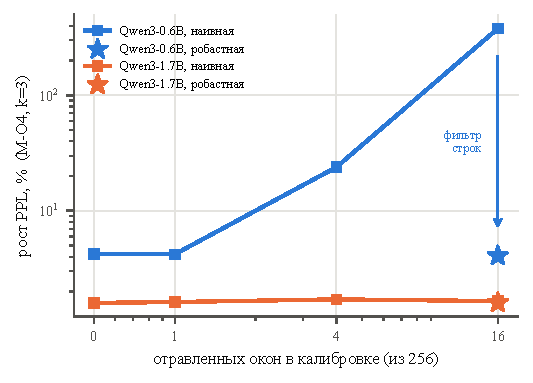
\includegraphics[width=0.55\linewidth]{figures/toggle.pdf}}
\caption{Рост PPL наивно откалиброванного M-O4 ($k=3$) в зависимости от
числа отравленных окон в калибровочной выборке из 256 окон; звёздочки "---
робастная калибровка при $n=16$.}
\label{fig:toggle}
\end{figure}

\subsection{Нейроны стока}

Массивную активацию позиции~0 создают единичные нейроны MLP слоя~2:
на Qwen3-0.6B пять нейронов дают 90\,\% вклада, на Qwen3-1.7B "--- один
нейрон 94\,\% (табл.~\ref{tab:sink}). Их удаление во всех позициях
уничтожает сток (норма $h_0$ падает с $6\,897$ до $429$ и с $14\,701$ до
$225$) и разрушает модель: $+54\,\%$ и $+231\,\%$ PPL. Удаление тех же
нейронов только на позициях $t \ge 1$ стоит $0.3\,\%$ и $0.0\,\%$, случайных
нейронов "--- ничего. Это объясняет, почему любой отбор нейронов в ранних
слоях обязан либо считать позицию~0 точно (как все наши MLP-замены), либо
защищать эти нейроны явно: в робастной статистике, исключающей позицию~0
и выбросы, нейрон стока невидим "--- вся его энергия сосредоточена именно
там. Полный A3 без точной позиции~0 с робастным отбором терял его и давал
$+556\,\%$ на 1.7B; с точной позицией~0 "--- $46\,\%$, как и наивный.
Нейроны стока "--- MLP-аналог <<супервесов>>~\cite{yu2024superweights}:
несколько параметров, без которых модель не работает.

\begin{table}[t]
\centering
\scriptsize
\setlength{\tabcolsep}{3pt}
\IfFileExists{tables/sink.tex}{\begin{tabular}{lcccrrrr}
\toprule
Модель & слой & нейронов & доля вклада в поз.~0 & \multicolumn{2}{c}{удалить везде} & удалить при $t\ge1$ & случайные \\
 & & & & $\Delta$PPL & $\|h_0\|$ после слоя & $\Delta$PPL & $\Delta$PPL \\
\midrule
Qwen3-0.6B & 2 & 5 & 90\% & +54.4\% & 429 & +0.3\% & -0.0\% \\
Qwen3-1.7B & 2 & 1 & 94\% & +230.9\% & 225 & +0.0\% & -0.0\% \\
\bottomrule
\end{tabular}
}{\textcolor{red}{[ожидает прогона]}}
\caption{Нейроны стока в слое $k_{\mathrm{sink}}-1$ и абляции (8 окон по
1024 токена): удаление во всех позициях, только при $t\ge1$ (позиция~0
точно) и такого же числа случайных нейронов.}
\label{tab:sink}
\end{table}

\subsection{Робастная калибровка}

Исправление детерминировано и бесплатно: из всех сумм по токенам
исключаются строки с $\|y_t\| > \tau \operatorname{med}_t \|y_t\|$,
$\tau = 10$ (правило не задевает ни одной обычной строки: доля токенов с
$\|z\|>10\,\mathrm{med}$ сверх выбросов равна нулю на обеих моделях), а в
критериях отбора нейронов "--- ещё и позиция~0 при точном её вычислении.
С робастной калибровкой обрыв исчезает (рис.~\ref{fig:howmany}): рост
PPL у M-O4 при $k=3$ составляет 4.7\,\% вместо 27.0\,\%, при $k=4$ "---
6.4 вместо 11.3, при $k=6$ "--- 8.7 вместо 13.0, при $k=8$ "--- 11.0 вместо
14.9, при $k=12$ "--- 14.7 вместо 19.3; у комбинации окно\,+\,M-O4 "--- 5.2,
7.5, 10.1, 13.6 и 22.2\,\% вместо 29.6, 13.1, 14.9, 18.1 и 27.6. Выигрыш
виден и на бенчмарках при $k=3$: средняя точность по семи задачам у
M-O4 растёт с 44.4 до 54.6\,\% при 54.9\,\% у исходной модели, у
окна\,+\,M-O4 "--- с 46.2 до 54.3\,\%. Та же поправка спасает M-O1 с
25\,\% точных нейронов (54.2 $\to$ 10.2\,\%) и табличную замену M-O2
(30.6 $\to$ 12.2\,\%). Робастная замкнутая форма оказывается сильнее
наивной калибровки с последующей дистилляцией: 300 шагов AdamW снижают
ошибку M-O1 лишь до 12.5\,\%.

\paragraph{Кого ловушка не касается.} Табл.~\ref{tab:robust} сравнивает
наивную и робастную калибровку для всех методов. Опубликованные методы
не страдают: SVD-LLM (12.8 против 12.6\,\%), ASVD (38.5 против 38.7\,\%)
и A3 (9.9 против 9.9\,\%) используют статистики для \emph{ранжирования}
или \emph{отбеливания}, а не как цели регрессии. Так, в матрице
$X^\top X$ входов down-проекции слоя~2, которую отбеливает SVD-LLM,
позиция~0 даёт $98.4\,\%$ следа, а среди позиций $\ge1$ один токен "---
$25.6\,\%$; но доминирующее направление лишь получает собственную
сингулярную компоненту и сохраняется при усечении. Страдают методы,
решающие задачу наименьших квадратов с целями в остаточном потоке: наши
M-O1, M-O2, M-O4 и, как показано ниже, корректоры на границе блоков.
Проверка на родных настройках SVD-LLM и ASVD (сжатие 10 и 20\,\%,
калибровка 256 окон по 2048 токенов, $k=3$) подтверждает это: наивная и
робастная статистики дают одинаковый результат (SVD-LLM 4.7/4.7 и
3.2/3.3\,\% на 0.6B, 1.5/1.5 и 0.9/0.9\,\% на 1.7B; ASVD 9.5/9.5 и 5.5/5.5,
4.9/4.9 и 3.0/3.0\,\%). Заметим, что при 20\,\% сжатия SVD-LLM стоит
столько же, сколько M-O4 при 75\,\% экономии MLP.

\begin{table}[t]
\centering
\small
\IfFileExists{tables/robust.tex}{\begin{tabular}{lrrrr}
\toprule
Метод & \multicolumn{2}{c}{наивная калибровка} & \multicolumn{2}{c}{робастная} \\
 & $\Delta$PPL & KL & $\Delta$PPL & KL \\
\midrule
SVD-LLM 50\% & 12.8\% & 0.138 & 12.6\% & 0.137 \\
ASVD 50\% & 38.5\% & 0.359 & 38.7\% & 0.361 \\
A3 FFN 50\% & 9.9\% & 0.114 & 9.9\% & 0.113 \\
A3 (блок) & 49.2\% & 0.433 & 49.5\% & 0.435 \\
M-O2: таблица по токену & 30.6\% & 0.288 & 12.2\% & 0.141 \\
M-O1: линейный + 25\% & 57.7\% & 0.480 & 10.2\% & 0.115 \\
M-O4: предиктор 25\% & 27.0\% & 0.268 & 4.7\% & 0.056 \\
Окно + M-O4 & 29.6\% & 0.286 & 5.2\% & 0.065 \\
\bottomrule
\end{tabular}
}{\textcolor{red}{[ожидает прогона]}}
\caption{Наивная и робастная калибровка при $k=k_{\mathrm{sink}}$
(Qwen3-0.6B, WikiText-2, 32 окна). Методы ранжирования и отбеливания
(SVD-LLM, ASVD, A3) не меняются; регрессионные замены меняются в
разы.}
\label{tab:robust}
\end{table}

\paragraph{Корректор на границе.} Оператор выравнивания активаций на
границе заменённого блока (ReplaceMe~\cite{shopkhoev2025replaceme},
Ghosted Layers~\cite{yun2026ghosted}) "--- та же регрессия. Подогнанный
наивно, он ухудшал наивный M-O4 (разд.~выше); подогнанный с исключением
строк-выбросов, он исправляет его: 27.0 $\to$ 4.8\,\% для полной карты
$d\times d$ и 4.7\,\% для карты, корректирующей только 8 каналов массивной
активации. На робастно откалиброванном M-O4 корректор ничего не добавляет
(4.7 $\to$ 4.7\,\%). Восьми каналов достаточно "--- прямое подтверждение
того, что вся ошибка ловушки лежит в направлении $r_o$.

\subsection{Стоки на токенах: второе семейство}
\label{sec:tokensinks}

У моделей архитектуры Llama правило <<сток "--- позиция~0>> оказывается
частным случаем более общего. На SmolLM2-1.7B массивную активацию
(норма $\approx 2\,900$ при медиане 33 после слоя~1) создаёт один нейрон
MLP слоя~1 (№\,4987, 68--89\,\% вклада) на токене <<\,the\,>> (а также на
первых кавычке и двойном переводе строки) в \emph{любой} позиции; сток
позиции~0 появляется лишь после слоя~7, и до него поздние слои используют
как стоки именно эти массивные токены. На Llama-3.2-1B массивную
активацию позиции~0 создают 12 нейронов MLP слоя~1 (90\,\% вклада);
их удаление во всех позициях стоит $+1\,353\,\%$ PPL, только при $t\ge1$
"--- $0.9\,\%$, у SmolLM2 64 нейрона слоя~7 (86\,\%) "--- $+2\,190$ и
$0.2\,\%$. Механизм тот же, что у Qwen3, но триггер иной.

Следствий два, и оба меняют замены. Во-первых, калиброванные замены MLP
без защиты рушатся даже с робастным фильтром строк по норме входа, потому
что массивные строки сидят в \emph{целях} регрессии на обычных токенах:
на SmolLM2 при $k=2$ M-O4 даёт $+123\,\%$, окно\,+\,M-O4 "--- $+612\,\%$.
Лечение детерминировано: нейроны стока находятся по калибровке априори
(токены с $\|\mathrm{MLP}(x)\|>20\,\mathrm{med}$, нейроны, покрывающие
90\,\% их вклада), всегда остаются в маске предиктора и отборе, у SVD
выносятся из факторизации и добавляются точно, а строки с большой
невязкой регрессии исключаются из подгонки (невязка нужна потому, что
окно внимания меняет набор токенов, становящихся массивными). После
этого M-O4 стоит $11.3\,\%$, окно\,+\,M-O4 "--- $13.9\,\%$, гребневая
замена "--- $15.3\,\%$; SVD-LLM остаётся непригодным (123\,\%). На
Qwen3 те же правки не меняют ни одного числа (4.7, 12.7 и 5.2\,\% при
$k=3$ на 0.6B), потому что там нейроны стока действуют только в позиции~0,
которая и так считается точно. Во-вторых, окно внимания должно хранить
массивные ключи в любой позиции: ключ считается стоком, если отношение
пика его каналов к среднему после RMSNorm превышает удвоенную медиану по
последовательности (априорное правило без калибровки). На SmolLM2 это
даёт $2.0\,\%$ вместо $13.7\,\%$ при $k=3$, $3.5$ вместо $62.4\,\%$ при
$k=6$ и $4.4$ вместо $64.1\,\%$ при $k=8$ ценой 0.2--4.4\,\% лишних
ключей; на Llama-3.2-1B "--- $2.8$ вместо $13.1\,\%$ при $k=2$; на Qwen3
ничего не портит: на 1.7B при $k=1..8$ кривая совпадает с позиционным стоком или чуть ниже
(5.5 вместо 5.7\,\% при $k=8$) при 0--0.1\,\% лишних ключей. Дозовый эксперимент на этом
семействе ловушку не включает (33.2--33.6\,\% при 0--16 отравленных окнах
на SmolLM2, 15.6--15.8\,\% на Llama-3.2-1B): отравление здесь не в
составе калибровки, а в самих данных, где массивные токены есть всегда.

\subsection{Вывод}

Любая калибровка в замкнутой форме, которая накапливает суммы по
токенам "--- гребневая регрессия, отбор нейронов по $\sum_t z_t^2$,
PCA входов "--- должна исключать позицию~0 и токены с массивной
активацией. Иначе ошибка приближения ложится в каналы стока и разрушает
механизм внимания ниже по потоку, причём ровно на том слое, где
появляется сток. Для квантования аналогичная роль каналов-выбросов
известна~\cite{yuan2023asvd}; здесь показано, что при структурной
замене блоков опасен не канал, а единичный токен в данных. В общем виде
правило звучит так: сток "--- это массивная активация, где бы она ни
возникла; позиция~0 у Qwen3 "--- частный случай, токен <<the>> у SmolLM2 "---
другой, и замена обязана сохранять и нейроны, создающие такие активации,
и ключи, которые их несут.

\section{Карта заменяемости и априорный критерий}\label{sec:criterion}

Кривые «первые $k$ слоёв» отвечают на вопрос о префиксе модели, но не
говорят, какие слои заменяемы вообще и можно ли это предсказать без
запуска замены. Для этого мы заменяем \emph{по одному} слою
$\ell = 0,\dots,27$ при неизменных остальных: внимание "--- окном 64 со
стоком, MLP "--- отбором 25\,\% нейронов по готовым активациям; для
сравнения на вход слоя $\ell$ подаётся гауссово возмущение с
относительной нормой 2\,\%. Качество "--- KL к исходной модели на 8 окнах
по 1024 токена. Параллельно на состояниях учителя считаются статистики,
не требующие замены: масса внимания вне окна (без стока), локальная
ошибка окна на выходе блока внимания, доля вклада 25\,\% сильнейших
нейронов в выход MLP и локальная ошибка их отбора.

\begin{figure}[t]
\centering
\figorpending{figures/map.pdf}{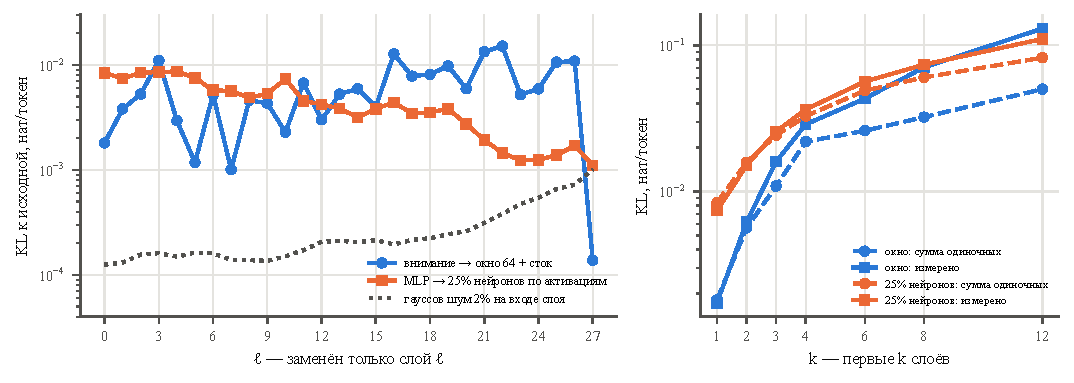
\includegraphics[width=\linewidth]{figures/map.pdf}}
\caption{Слева "--- карта заменяемости Qwen3-0.6B: KL при замене только
слоя $\ell$ (внимание "--- окно 64 + сток; MLP "--- 25\,\% нейронов) и при
изотропном шуме 2\,\% на его входе. Справа "--- аддитивность: сумма KL
одиночных замен первых $k$ слоёв против измеренного KL при их
одновременной замене.}
\label{fig:map}
\end{figure}

\begin{table}[t]
\centering
\small
\IfFileExists{tables/criterion.tex}{\begin{tabular}{llc}
\toprule
Блок & Статистика (без запуска замены) & Спирмен с KL \\
\midrule
Внимание & масса внимания вне окна & 0.37 \\
 & локальная ошибка окна (отн. выхода внимания) & 0.82 \\
 & ошибка относительно остаточного потока & 0.52 \\
 & то же $\times$ чувствительность слоя & 0.77 \\
MLP & $1-$ доля вклада 25\% сильнейших нейронов & 0.92 \\
 & локальная ошибка отбора (отн. выхода MLP) & 0.82 \\
 & ошибка относительно остаточного потока & 0.97 \\
 & то же $\times$ чувствительность слоя & 0.96 \\
\bottomrule
\end{tabular}
}{\textcolor{red}{[ожидает прогона]}}
\caption{Ранговая корреляция Спирмена (28 слоёв) между статистиками
слоя, вычисленными без замены, и KL при его одиночной замене.}
\label{tab:criterion}
\end{table}

\paragraph{Карта по глубине.} Для внимания KL одиночной замены меняется
на два порядка по глубине и немонотонно: легче всего заменяются слои
27, 7, 5, 0, 10 и 4 ($\mathrm{KL} \le 0.003$), труднее всего "--- 22, 21
и 16 ($\ge 0.013$); слой-сток 3 оказывается одним из трудных (0.011),
так как помимо стока содержит головы с дальним контекстом. Для MLP
картина противоположна исходной посылке о «простых первых слоях»:
KL максимален в слоях 0--4 (0.0084--0.0087) и минимален в слоях 21--27
(0.0011--0.0019). Иными словами, MLP первых слоёв "--- самые
\emph{незаменяемые} отбором нейронов во всей модели, а поздних "--- самые
заменяемые; это согласуется с ростом разреженности активаций по глубине
и с ролью ранних MLP как «детокенизатора»~\cite{elhage2021framework}.

\paragraph{Априорный критерий.} Для MLP достаточно одной статистики: доля
вклада 25\,\% сильнейших нейронов предсказывает KL одиночной замены с
корреляцией 0.92, а локальная ошибка отбора, отнесённая к норме
остаточного потока, "--- 0.97 (табл.~\ref{tab:criterion}). Для внимания
масса вне окна предсказывает плохо (0.37): важно не то, сколько массы
теряется, а как меняется выход блока; локальная ошибка окна даёт 0.82.

\paragraph{Воспроизводимость на 1.7B.} Все три наблюдения повторяются
на Qwen3-1.7B без подгонки: корреляции Спирмена составляют 0.91--0.96 для
MLP и 0.33--0.77 для внимания; карта по глубине почти та же (внимание
легче всего заменяется в слоях 27, 5, 7, 10, 0, труднее всего "--- в 21,
22 и слое-стоке 3; MLP слоёв 21--27 заменяется в 15--20 раз легче, чем
слоёв 3--5); сумма одиночных KL совпадает с измеренной для отбора
нейронов (0.043 против 0.050 при $k=8$) и занижает её для окна (0.035
против 0.066).

\paragraph{Аддитивность и направление ошибки.} Для отбора нейронов сумма
KL одиночных замен первых $k$ слоёв почти совпадает с измеренным KL при
их совместной замене (0.024 против 0.026 при $k=3$, 0.082 против 0.111
при $k=12$). Для окна сумма занижает: 0.011 против 0.016 при $k=3$ и
0.050 против 0.130 при $k=12$, то есть ошибки окна взаимодействуют и
накапливаются суперaддитивно. Та же разница видна по отношению KL к
энергии возмущения: ошибка окна вредит в 2--6 раз сильнее изотропного
шума той же энергии на том же слое, а ошибка отбора нейронов ведёт себя
как шум (отношение 0.9--1.6). Прямое измерение структуры ошибок
подтверждает это: ковариация ошибки на выходе модели при замене окном
имеет эффективный ранг 19--115 (на 8 главных компонент приходится
20--44\,\% энергии), при отборе нейронов "--- 83--277 (11--23\,\%); средний
косинус между ошибками от замен разных слоёв равен 0.071 для окна против
0.022 для MLP (0.135 против 0.034 среди первых шести слоёв). Ошибки окна
низкоранговы и согласованы между слоями "--- они складываются; ошибки
отбора нейронов близки к изотропному шуму и складываются по энергии.

\paragraph{CATS не работает в ранних слоях.} Пороговый отбор по величине
$|\mathrm{act}(\mathrm{gate})|$~\cite{lee2024cats}, который в литературе
применяют ко всей модели, в одиночной замене слоя проигрывает отбору по
полному вкладу нейрона в 5--37 раз в слоях 0--5 и лишь в 1.3--3 раза в
слоях 22--27 (рис.~\ref{fig:cats}); на 1.7B "--- в 2.5--5.6 и 1.3--3 раза.
При замене первых трёх слоёв CATS с 25\,\% активных нейронов даёт
$+70\,\%$ PPL, при $k=4$ "--- почти $+300\,\%$. В ранних слоях важен
критерий отбора, и именно там дешёвые пороговые методы не применимы.

\begin{figure}[t]
\centering
\figorpending{figures/cats_depth.pdf}{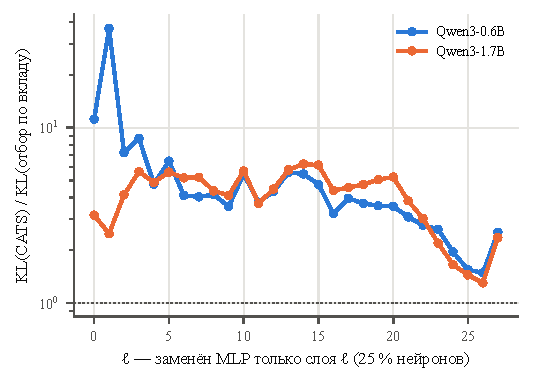
\includegraphics[width=0.5\linewidth]{figures/cats_depth.pdf}}
\caption{Отношение KL при пороговом отборе CATS к KL при отборе 25\,\%
нейронов по вкладу, замена MLP одного слоя $\ell$.}
\label{fig:cats}
\end{figure}

\paragraph{Почему MLP ранних слоёв незаменим.} Карта фиксирует факт, а
не причину. Мы сопоставили KL одиночной замены MLP с пятью свойствами
слоя, измеренными на состояниях учителя (Qwen3-0.6B). Сильнее всего с KL
связана концентрация вклада (доля 25\,\% сильнейших нейронов, Спирмен
$-0.92$) и число существенно активных нейронов (вклад выше $1\,\%$ от
максимального по токену, Спирмен $+0.70$): в слоях 0--5 активны
$1\,900$--$2\,300$ нейронов из $3\,072$, в слоях 21--26 "--- $1\,200$--$1\,400$,
в слое 27 "--- 275. Второй фактор "--- величина записи: норма выхода MLP
относительно остаточного потока равна $0.45$--$0.72$ в слоях 0--4 и
$0.22$--$0.40$ в слоях 11--26 (Спирмен $+0.44$); эффективный ранг выхода
ведёт себя так же ($+0.52$). Гипотеза о том, что ранние MLP пишут именно
в подпространство, которое читают ключи и запросы слоя-стока, не
подтвердилась: доля их выхода в этом подпространстве ($0.74$) совпадает
со случайным подпространством той же размерности ($0.78$). Наконец,
ошибка отбора на продолжениях слов выше, чем на началах, только в слоях
0--5 ($0.18$--$0.22$ против $0.14$--$0.19$), а с седьмого слоя разницы нет.
Итог: MLP ранних слоёв пишет в остаточный поток большие, плотные и
высокоранговые векторы "--- в особенности когда собирает слово из
нескольких токенов, "--- и любое подмножество нейронов теряет заметную долю
такого вектора; MLP поздних слоёв разрежен и мал относительно уже
большого остаточного потока, поэтому его легко заменить.
На Qwen3-1.7B все три зависимости повторяются (ранговая корреляция концентрации
вклада с KL замены $-0.91$, доли активных нейронов $+0.75$); на SmolLM2 они
слабеют "--- см. абзац <<Второе семейство>> ниже.

\paragraph{Что не покрывается словарём.} Разбиение ошибки остаточного
потока на входе слоя~3 по типам токенов показывает, чего не хватает
каждой замене. Табличная замена MLP по токену (M-O2, робастная; средняя
относительная ошибка 0.31) хуже всего на продолжениях слов (0.59 против
0.25--0.30 для пунктуации, начал слов и цифр), и десять худших токенов "---
это фрагменты вроде <<se>>, <<ga>>, <<ter>>, <<ly>>: сборка слова из
кусков требует контекста соседей, которого у таблицы нет. У предиктора
нейронов M-O4 (0.21) тот же профиль в смягчённом виде (0.41 на
продолжениях). Окно (0.11), напротив, одинаково хорошо справляется с
началами и продолжениями слов (0.09--0.10), а хуже всего "--- на переводах
строки и разделителях (0.17--0.27): редкие структурные токены, которым
нужен далёкий контекст. Иными словами, первые слои делают две разные
вещи: локальную сборку слов из кусков, которую окно сохраняет, а словарь
теряет, и разметку структуры документа, для которой нужен хвост
контекста.

\subsection{Планировщик замен по априорным статистикам}

Критерий позволяет выбирать, \emph{что} заменять, не запуская замены.
Мы подгоняем на Qwen3-0.6B две лог-линейные зависимости KL одиночной
замены от статистик (локальная ошибка окна для внимания; ошибка отбора
относительно остаточного потока для MLP) и показатель суперaддитивности
внимания $\gamma=0.47$ по кривой howmany, затем применяем их к
Qwen3-1.7B \emph{по её собственным статистикам}: предсказанные KL
одиночных замен коррелируют с измеренными на уровне 0.75 (внимание) и
0.94 (MLP). Жадный план из $m$ компонент с минимальным предсказанным
итогом сравнивается с двумя префиксами: первые $m/2$ слоёв целиком и
окно в первых $m$ слоях (рис.~\ref{fig:planner}). При $m=6$ план даёт
KL $0.0031$ ($+0.1\,\%$ PPL) против $0.0335$ ($+3.2\,\%$) и $0.0453$
($+4.0\,\%$); при $m=12$ "--- $0.0070$ ($+0.4\,\%$) против $0.083$ и
$0.114$. План состоит из MLP поздних слоёв (23--27) и внимания слоя~0, то
есть критерий сам уводит замену от префикса в хвост модели. На 0.6B
(подгонка и проверка на одной модели) выигрыш тот же: при $m=12$ "---
$2.2\,\%$ против $9.5$ и $13.9\,\%$.

\begin{figure}[t]
\centering
\figorpending{figures/planner.pdf}{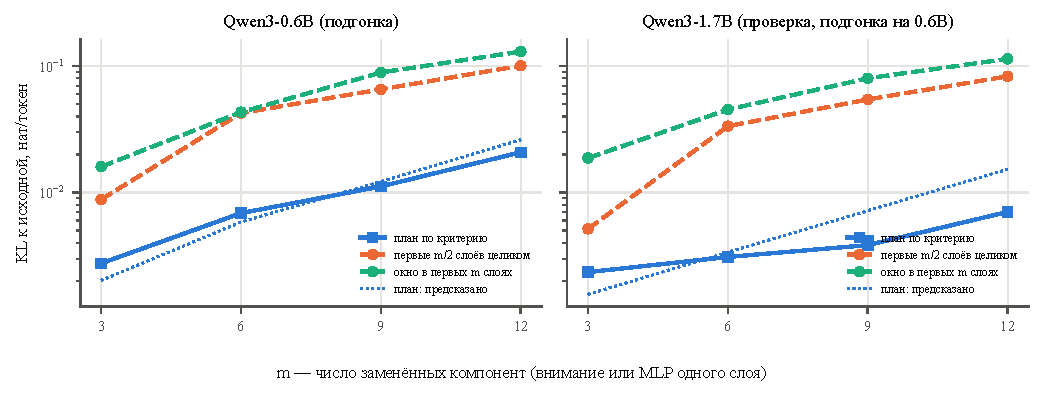
\includegraphics[width=\linewidth]{figures/planner.pdf}}
\caption{Планировщик по априорным статистикам против замены префикса:
KL в зависимости от числа заменённых компонент $m$. Зависимости
подогнаны на Qwen3-0.6B (слева) и без изменений применены к Qwen3-1.7B
(справа); пунктир "--- предсказание плана.}
\label{fig:planner}
\end{figure}

\paragraph{Второе семейство.} Те же зависимости, подогнанные на
Qwen3-0.6B, применены без изменений к SmolLM2-1.7B и Llama-3.2-1B по их
собственным статистикам. Планировщик переносится: на SmolLM2 при $m=6$
план даёт KL 0.026 ($+2.6\,\%$ PPL) против 0.145 ($+15.8\,\%$) у префикса
из трёх блоков и 0.49 ($+62\,\%$) у окна в шести первых слоях (с
позиционным стоком); план состоит из внимания слоёв 0, 22, 23 и MLP
слоёв 20--22, то есть снова уходит из начала модели. На Llama-3.2-1B при
$m=6$ "--- $7.9\,\%$ против 20.7 и 22.3\,\%, при $m=12$ "--- 28.1 против
35.7 и 47.2\,\%; при $m=3$ префикс из блока~0 целиком ($3.2\,\%$) лучше
плана ($4.6\,\%$): у 16-слойной модели предсказание KL внимания
завышено. Критерий для MLP переносится хуже: ранговая корреляция
концентрации вклада с KL замены составляет $-0.25$ на SmolLM2 и $-0.51$
на Llama-3.2-1B против $-0.91$ на Qwen3-1.7B, а поздние MLP у SmolLM2 не
дешевле ранних (KL одиночной замены 0.004--0.0075 по всей глубине, слой~23
"--- самый дорогой), тогда как у Qwen3 они в 5--30 раз дешевле. Сравнение
CATS с отбором по вкладу (отношение ошибок 1.8--3.7 по всем 24 слоям) и
аддитивность воспроизводятся.

% Обсуждение и ограничения (main.tex)
\section{Обсуждение и ограничения}\label{sec:discussion}

\paragraph{Связь с дискуссией о <<чистоте>> сетей.}
Замена слоя явным алгоритмом с малым KL "--- конструктивная форма
утверждения <<мы понимаем, что делает этот слой>> в смысле критерия
Gao~\cite{gao_notclean}. По этому критерию первые слои Qwen3 <<чисты>>
наполовину: их внимание действительно локально и сводится к окну с
потерей 1.5--1.8\,\% PPL, а их MLP "--- нет: лучшая явная замена с
предсказанием нейронов стоит 4.7\,\% на 0.6B и 1.7\,\% на 1.7B, табличная
замена по токену "--- 12\,\%, линейная "--- 20\,\%. При этом MLP поздних
слоёв по карте заменяемости в 15--20 раз <<чище>> ранних. Иными словами,
простота первых слоёв "--- свойство их внимания, а не их MLP.

\paragraph{Четыре практических правила.} Из результатов следуют правила
для любой пост-хок замены блоков в замкнутой форме: (1) суммы по токенам
не должны включать строки с массивной активацией "--- одна такая строка
в калибровке доминирует в задаче наименьших квадратов, а порог опасности
лежит между одним и четырьмя окнами из 256; (2) сток "--- это массивная активация, где бы она ни возникла:
нейроны, создающие её, должны сохраняться явно, а окно внимания "---
хранить несущие её ключи; у Qwen3 это позиция~0, у Llama-семейства "---
ещё и токены вроде <<the>> в любой позиции, и без этого правила окно
стоит 64\,\% вместо 4\,\% на SmolLM2; (3) выбирать блок для замены
надо по измеренной чувствительности, а не по косинусной близости
состояний: на Qwen3-0.6B косинусный критерий ошибается в 4--5 раз;
(4) калибровать надо на смеси доменов "--- иначе ошибка калиброванной
замены вне домена втрое выше.

\paragraph{Ограничения.}
\begin{itemize}
  \item Ускорение оценивается по числу операций. Измеренное время
    (табл.~\ref{tab:timing}) показывает, что без специализированного
    ядра окна реализация на чистом PyTorch медленнее fused-ядра полного
    внимания; экономия в несколько процентов умножений на первых слоях
    сама по себе ускорения не даёт, выигрыш окна "--- память кэша
    ключей-значений на длинном контексте.
  \item Калибровка на одном домене переобучает калиброванные замены MLP
    (ошибка вне домена втрое выше); смешанная калибровка выравнивает
    ошибку ценой роста внутри домена.
  \item Исследованы два семейства (Qwen3-0.6B/1.7B, SmolLM2-1.7B,
    Llama-3.2-1B) размером до 1.7B; вычисления выполнены на ноутбуке.
    Выводы о внимании и о стоках повторяются на обоих семействах, выводы о
    заменимости MLP и об априорном критерии для MLP "--- нет: у
    Llama-семейства первый MLP дороже, а концентрация вклада предсказывает
    KL слабее. Вопрос о сохранении <<обменного курса>> с ростом размера
    требует моделей 4B--32B. Кривые по $k$ для Llama-3.2-1B и точки окна с
    массивными стоками при всех $k$ досчитываются; в таблицах они
    отмечены.
  \item Бенчмарки посчитаны на подвыборках: по 200 примеров для всех
    столбцов ($\pm2.5$ п.п. для среднего по семи задачам) и по 1000 для
    главных ($\pm1.1$ п.п.); интервалы для PPL и KL даны по бутстрэпу окон.
  \item Дистилляционный контроль (300 шагов AdamW) ограничен шестью
    методами и малым числом шагов; для метода O4 он расходится.
  \item Методы из литературы адаптированы к Qwen3 (A3) или взяты в
    детерминированной части (SVD-LLM без дообучения, Deja Vu в
    оракульном режиме, MoEfication без обучаемого маршрутизатора). Их
    обучаемые варианты оценены только в дистилляционном контроле.
\end{itemize}

\section{Заключение}
Мы спросили, можно ли заменить первые слои готовой LLM явными
детерминированными алгоритмами, и получили ответ в четырёх частях.
Внимание первых слоёв "--- да: окно из 64 позиций со стоком заменяет
первые три слоя Qwen3-0.6B и 1.7B с ростом PPL 1.5--1.8\,\% и без изменения
точности на бенчмарках, первые шесть "--- в пределах 5\,\%, и число стоков,
как и длина контекста до 8 тыс. токенов, на это почти не влияют. MLP
первых слоёв "--- лишь частично: предсказание 25\,\% активных нейронов в
замкнутой форме (M-O4) стоит 4.7 и 1.7\,\% PPL при стоимости $0.3$ MLP,
тогда как пороговый отбор, линейные карты и низкоранговые приближения
теряют в разы больше, а по карте заменяемости MLP ранних слоёв "--- самые
незаменимые во всей модели. Любая калибровка в замкнутой форме "--- только
с защитой от массивных активаций: одна строка данных отравляет регрессию
(что мы доказали формулой, воспроизвели дозой и вылечили исключением
строк), а один нейрон, создающий сток, должен быть сохранён. Второе
семейство показало общий вид этого правила: сток "--- массивная
активация, у SmolLM2 её создаёт один нейрон на токене <<the>> в любой
позиции, и только защита таких нейронов и хранение таких ключей делают
замены переносимыми (окно: 64 $\to$ 4\,\%; M-O4: 123 $\to$ 11\,\%). Наконец,
дешёвые априорные статистики предсказывают заменяемость слоёв и на
непросмотренной модели выбирают план замен в 10--15 раз лучше префикса.
Все замены укладываются в один обменный курс "--- около процента PPL за
процент вычислений на 0.6B и вдвое лучше на 1.7B, "--- и проверка того,
продолжает ли курс улучшаться с размером, составляет следующий шаг.


% Общий список литературы (подключается через % Общий список литературы (подключается через % Общий список литературы (подключается через \input{references})
% Нумерация совпадает с literature.md
\begin{thebibliography}{99}
\selectlanguage{english}

\bibitem{elhage2021framework}
N.~Elhage et al. A Mathematical Framework for Transformer Circuits.
Transformer Circuits Thread, 2021.
\url{https://transformer-circuits.pub/2021/framework/index.html}

\bibitem{vaswani2017attention}
A.~Vaswani et al. Attention Is All You Need. NeurIPS, 2017.
arXiv:1706.03762.

\bibitem{geva2021ffn}
M.~Geva et al. Transformer Feed-Forward Layers Are Key-Value Memories.
EMNLP, 2021. arXiv:2012.14913.

\bibitem{cordonnier2020relationship}
J.-B.~Cordonnier et al. On the Relationship between Self-Attention and
Convolutional Layers. ICLR, 2020. arXiv:1911.03584.

\bibitem{dong2021attention}
Y.~Dong et al. Attention is Not All You Need: Pure Attention Loses Rank
Doubly Exponentially with Depth. ICML, 2021. arXiv:2103.03404.

\bibitem{cammarata_clean}
N.~Cammarata. Neural Networks Are Already Clean. Goodfire, 2026.
\url{https://already-clean.goodfire.com/}

\bibitem{gao_notclean}
L.~Gao. Neural networks are not already clean. LessWrong, 2026.
\url{https://www.lesswrong.com/posts/Dkh7pXKjoNWkkxQDz/neural-networks-are-not-already-clean}

\bibitem{olah2020zoom}
C.~Olah et al. Zoom In: An Introduction to Circuits. Distill, 2020.
\url{https://distill.pub/2020/circuits/zoom-in/}

\bibitem{lissack_clean}
M.~Lissack. Already Clean, Not Yet Meaningful: One ``how'' for the
question Cammarata has opened. PhilArchive.
\url{https://philarchive.org/rec/LISACN} % TODO: год

\bibitem{ibm_clean}
S.~Brodsky. Is AI easier to understand than scientists thought? IBM Think, 2026.
\url{https://www.ibm.com/think/news/is-ai-easier-to-understand-than-scientists-thought-goodfire-essay}

\bibitem{katharopoulos2020rnn}
A.~Katharopoulos et al. Transformers are RNNs: Fast Autoregressive
Transformers with Linear Attention. ICML, 2020. arXiv:2006.16236.

\bibitem{wang2020linformer}
S.~Wang et al. Linformer: Self-Attention with Linear Complexity, 2020.
arXiv:2006.04768.

\bibitem{xiong2021nystrom}
Y.~Xiong et al. Nyströmformer: A Nyström-Based Algorithm for
Approximating Self-Attention. AAAI, 2021. arXiv:2102.03902.

\bibitem{choromanski2021performer}
K.~Choromanski et al. Rethinking Attention with Performers. ICLR, 2021.
arXiv:2009.14794.

\bibitem{peng2021rfa}
H.~Peng et al. Random Feature Attention. ICLR, 2021. arXiv:2103.02143.

\bibitem{lu2021soft}
J.~Lu et al. SOFT: Softmax-free Transformer with Linear Complexity.
NeurIPS, 2021. arXiv:2110.11945.

\bibitem{child2019sparse}
R.~Child et al. Generating Long Sequences with Sparse Transformers, 2019.
arXiv:1904.10509.

\bibitem{kitaev2020reformer}
N.~Kitaev et al. Reformer: The Efficient Transformer. ICLR, 2020.
arXiv:2001.04451.

\bibitem{zaheer2020bigbird}
M.~Zaheer et al. Big Bird: Transformers for Longer Sequences. NeurIPS,
2020. arXiv:2007.14062.

\bibitem{leethorp2022fnet}
J.~Lee-Thorp et al. FNet: Mixing Tokens with Fourier Transforms.
NAACL, 2022. arXiv:2105.03824.

\bibitem{tay2021synthesizer}
Y.~Tay et al. Synthesizer: Rethinking Self-Attention in Transformer
Models. ICML, 2021. arXiv:2005.00743.

\bibitem{wong2025a3}
J.~T.~H.~Wong et al. A3: an Analytical Low-Rank Approximation Framework
for Attention, 2025. arXiv:2505.12942.

\bibitem{olsson2022induction}
C.~Olsson et al. In-context Learning and Induction Heads. Transformer
Circuits Thread, 2022. arXiv:2209.11895.

\bibitem{bricken2023monosemanticity}
T.~Bricken et al. Towards Monosemanticity: Decomposing Language Models
With Dictionary Learning. Transformer Circuits Thread, 2023.
\url{https://transformer-circuits.pub/2023/monosemantic-features/index.html}

\bibitem{rai2024review}
D.~Rai et al. A Practical Review of Mechanistic Interpretability for
Transformer-Based Language Models, 2024. arXiv:2407.02646.

\bibitem{yuan2023asvd}
Z.~Yuan et al. ASVD: Activation-aware Singular Value Decomposition for
Compressing Large Language Models, 2023. arXiv:2312.05821.

\bibitem{wang2025svdllm}
X.~Wang et al. SVD-LLM: Truncation-aware Singular Value Decomposition for
Large Language Model Compression. ICLR, 2025. arXiv:2403.07378.

\bibitem{liu2023dejavu}
Z.~Liu et al. Deja Vu: Contextual Sparsity for Efficient LLMs at Inference
Time. ICML, 2023. arXiv:2310.17157.

\bibitem{zhang2022moefication}
Z.~Zhang et al. MoEfication: Transformer Feed-forward Layers are Mixtures of
Experts. Findings of ACL, 2022. arXiv:2110.01786.

\bibitem{lee2024cats}
J.-Y.~Lee et al. CATS: Contextually-Aware Thresholding for Sparsity in Large
Language Models. COLM, 2024. arXiv:2404.08763.

\bibitem{liu2024teal}
J.~Liu et al. Training-Free Activation Sparsity in Large Language Models.
ICLR, 2025. arXiv:2408.14690.

\bibitem{shopkhoev2025replaceme}
D.~Shopkhoev et al. ReplaceMe: Network Simplification via Depth Pruning and
Transformer Block Linearization. NeurIPS, 2025. arXiv:2505.02819.

\bibitem{yun2026ghosted}
V.-D.~Yun et al. Ghosted Layers: Unconstrained Activation Alignment for
Recovering Layer-Pruned LLMs. ICML, 2026. arXiv:2605.15491.

\bibitem{yu2024superweights}
M.~Yu et al. The Super Weight in Large Language Models. arXiv:2411.07191,
2024.

\bibitem{sun2024massive}
M.~Sun et al. Massive Activations in Large Language Models. COLM, 2024.
arXiv:2402.17762.

\bibitem{merity2017pointer}
S.~Merity, C.~Xiong, J.~Bradbury, R.~Socher. Pointer Sentinel Mixture Models. ICLR, 2017.
arXiv:1609.07843. Набор WikiText: \url{https://huggingface.co/datasets/Salesforce/wikitext}

\bibitem{gao2020pile}
L.~Gao et al. The Pile: An 800GB Dataset of Diverse Text for Language Modeling. 2020.
arXiv:2101.00027. Подвыборка pile-10k: \url{https://huggingface.co/datasets/NeelNanda/pile-10k}

\bibitem{gao2023harness}
L.~Gao et al. A framework for few-shot language model evaluation (lm-evaluation-harness), v0.4. Zenodo, 2023.
\url{https://github.com/EleutherAI/lm-evaluation-harness}

\bibitem{paperno2016lambada}
D.~Paperno et al. The LAMBADA dataset: Word prediction requiring a broad discourse context. ACL, 2016.

\bibitem{zellers2019hellaswag}
R.~Zellers, A.~Holtzman, Y.~Bisk, A.~Farhadi, Y.~Choi. HellaSwag: Can a Machine Really Finish Your Sentence? ACL, 2019.

\bibitem{clark2018arc}
P.~Clark et al. Think you have Solved Question Answering? Try ARC, the AI2 Reasoning Challenge. 2018. arXiv:1803.05457.

\bibitem{bisk2020piqa}
Y.~Bisk, R.~Zellers, R.~Le~Bras, J.~Gao, Y.~Choi. PIQA: Reasoning about Physical Commonsense in Natural Language. AAAI, 2020.

\bibitem{sakaguchi2020winogrande}
K.~Sakaguchi, R.~Le~Bras, C.~Bhagavatula, Y.~Choi. WinoGrande: An Adversarial Winograd Schema Challenge at Scale. AAAI, 2020.

\bibitem{hendrycks2021mmlu}
D.~Hendrycks et al. Measuring Massive Multitask Language Understanding. ICLR, 2021. arXiv:2009.03300.

\end{thebibliography}
)
% Нумерация совпадает с literature.md
\begin{thebibliography}{99}
\selectlanguage{english}

\bibitem{elhage2021framework}
N.~Elhage et al. A Mathematical Framework for Transformer Circuits.
Transformer Circuits Thread, 2021.
\url{https://transformer-circuits.pub/2021/framework/index.html}

\bibitem{vaswani2017attention}
A.~Vaswani et al. Attention Is All You Need. NeurIPS, 2017.
arXiv:1706.03762.

\bibitem{geva2021ffn}
M.~Geva et al. Transformer Feed-Forward Layers Are Key-Value Memories.
EMNLP, 2021. arXiv:2012.14913.

\bibitem{cordonnier2020relationship}
J.-B.~Cordonnier et al. On the Relationship between Self-Attention and
Convolutional Layers. ICLR, 2020. arXiv:1911.03584.

\bibitem{dong2021attention}
Y.~Dong et al. Attention is Not All You Need: Pure Attention Loses Rank
Doubly Exponentially with Depth. ICML, 2021. arXiv:2103.03404.

\bibitem{cammarata_clean}
N.~Cammarata. Neural Networks Are Already Clean. Goodfire, 2026.
\url{https://already-clean.goodfire.com/}

\bibitem{gao_notclean}
L.~Gao. Neural networks are not already clean. LessWrong, 2026.
\url{https://www.lesswrong.com/posts/Dkh7pXKjoNWkkxQDz/neural-networks-are-not-already-clean}

\bibitem{olah2020zoom}
C.~Olah et al. Zoom In: An Introduction to Circuits. Distill, 2020.
\url{https://distill.pub/2020/circuits/zoom-in/}

\bibitem{lissack_clean}
M.~Lissack. Already Clean, Not Yet Meaningful: One ``how'' for the
question Cammarata has opened. PhilArchive.
\url{https://philarchive.org/rec/LISACN} % TODO: год

\bibitem{ibm_clean}
S.~Brodsky. Is AI easier to understand than scientists thought? IBM Think, 2026.
\url{https://www.ibm.com/think/news/is-ai-easier-to-understand-than-scientists-thought-goodfire-essay}

\bibitem{katharopoulos2020rnn}
A.~Katharopoulos et al. Transformers are RNNs: Fast Autoregressive
Transformers with Linear Attention. ICML, 2020. arXiv:2006.16236.

\bibitem{wang2020linformer}
S.~Wang et al. Linformer: Self-Attention with Linear Complexity, 2020.
arXiv:2006.04768.

\bibitem{xiong2021nystrom}
Y.~Xiong et al. Nyströmformer: A Nyström-Based Algorithm for
Approximating Self-Attention. AAAI, 2021. arXiv:2102.03902.

\bibitem{choromanski2021performer}
K.~Choromanski et al. Rethinking Attention with Performers. ICLR, 2021.
arXiv:2009.14794.

\bibitem{peng2021rfa}
H.~Peng et al. Random Feature Attention. ICLR, 2021. arXiv:2103.02143.

\bibitem{lu2021soft}
J.~Lu et al. SOFT: Softmax-free Transformer with Linear Complexity.
NeurIPS, 2021. arXiv:2110.11945.

\bibitem{child2019sparse}
R.~Child et al. Generating Long Sequences with Sparse Transformers, 2019.
arXiv:1904.10509.

\bibitem{kitaev2020reformer}
N.~Kitaev et al. Reformer: The Efficient Transformer. ICLR, 2020.
arXiv:2001.04451.

\bibitem{zaheer2020bigbird}
M.~Zaheer et al. Big Bird: Transformers for Longer Sequences. NeurIPS,
2020. arXiv:2007.14062.

\bibitem{leethorp2022fnet}
J.~Lee-Thorp et al. FNet: Mixing Tokens with Fourier Transforms.
NAACL, 2022. arXiv:2105.03824.

\bibitem{tay2021synthesizer}
Y.~Tay et al. Synthesizer: Rethinking Self-Attention in Transformer
Models. ICML, 2021. arXiv:2005.00743.

\bibitem{wong2025a3}
J.~T.~H.~Wong et al. A3: an Analytical Low-Rank Approximation Framework
for Attention, 2025. arXiv:2505.12942.

\bibitem{olsson2022induction}
C.~Olsson et al. In-context Learning and Induction Heads. Transformer
Circuits Thread, 2022. arXiv:2209.11895.

\bibitem{bricken2023monosemanticity}
T.~Bricken et al. Towards Monosemanticity: Decomposing Language Models
With Dictionary Learning. Transformer Circuits Thread, 2023.
\url{https://transformer-circuits.pub/2023/monosemantic-features/index.html}

\bibitem{rai2024review}
D.~Rai et al. A Practical Review of Mechanistic Interpretability for
Transformer-Based Language Models, 2024. arXiv:2407.02646.

\bibitem{yuan2023asvd}
Z.~Yuan et al. ASVD: Activation-aware Singular Value Decomposition for
Compressing Large Language Models, 2023. arXiv:2312.05821.

\bibitem{wang2025svdllm}
X.~Wang et al. SVD-LLM: Truncation-aware Singular Value Decomposition for
Large Language Model Compression. ICLR, 2025. arXiv:2403.07378.

\bibitem{liu2023dejavu}
Z.~Liu et al. Deja Vu: Contextual Sparsity for Efficient LLMs at Inference
Time. ICML, 2023. arXiv:2310.17157.

\bibitem{zhang2022moefication}
Z.~Zhang et al. MoEfication: Transformer Feed-forward Layers are Mixtures of
Experts. Findings of ACL, 2022. arXiv:2110.01786.

\bibitem{lee2024cats}
J.-Y.~Lee et al. CATS: Contextually-Aware Thresholding for Sparsity in Large
Language Models. COLM, 2024. arXiv:2404.08763.

\bibitem{liu2024teal}
J.~Liu et al. Training-Free Activation Sparsity in Large Language Models.
ICLR, 2025. arXiv:2408.14690.

\bibitem{shopkhoev2025replaceme}
D.~Shopkhoev et al. ReplaceMe: Network Simplification via Depth Pruning and
Transformer Block Linearization. NeurIPS, 2025. arXiv:2505.02819.

\bibitem{yun2026ghosted}
V.-D.~Yun et al. Ghosted Layers: Unconstrained Activation Alignment for
Recovering Layer-Pruned LLMs. ICML, 2026. arXiv:2605.15491.

\bibitem{yu2024superweights}
M.~Yu et al. The Super Weight in Large Language Models. arXiv:2411.07191,
2024.

\bibitem{sun2024massive}
M.~Sun et al. Massive Activations in Large Language Models. COLM, 2024.
arXiv:2402.17762.

\bibitem{merity2017pointer}
S.~Merity, C.~Xiong, J.~Bradbury, R.~Socher. Pointer Sentinel Mixture Models. ICLR, 2017.
arXiv:1609.07843. Набор WikiText: \url{https://huggingface.co/datasets/Salesforce/wikitext}

\bibitem{gao2020pile}
L.~Gao et al. The Pile: An 800GB Dataset of Diverse Text for Language Modeling. 2020.
arXiv:2101.00027. Подвыборка pile-10k: \url{https://huggingface.co/datasets/NeelNanda/pile-10k}

\bibitem{gao2023harness}
L.~Gao et al. A framework for few-shot language model evaluation (lm-evaluation-harness), v0.4. Zenodo, 2023.
\url{https://github.com/EleutherAI/lm-evaluation-harness}

\bibitem{paperno2016lambada}
D.~Paperno et al. The LAMBADA dataset: Word prediction requiring a broad discourse context. ACL, 2016.

\bibitem{zellers2019hellaswag}
R.~Zellers, A.~Holtzman, Y.~Bisk, A.~Farhadi, Y.~Choi. HellaSwag: Can a Machine Really Finish Your Sentence? ACL, 2019.

\bibitem{clark2018arc}
P.~Clark et al. Think you have Solved Question Answering? Try ARC, the AI2 Reasoning Challenge. 2018. arXiv:1803.05457.

\bibitem{bisk2020piqa}
Y.~Bisk, R.~Zellers, R.~Le~Bras, J.~Gao, Y.~Choi. PIQA: Reasoning about Physical Commonsense in Natural Language. AAAI, 2020.

\bibitem{sakaguchi2020winogrande}
K.~Sakaguchi, R.~Le~Bras, C.~Bhagavatula, Y.~Choi. WinoGrande: An Adversarial Winograd Schema Challenge at Scale. AAAI, 2020.

\bibitem{hendrycks2021mmlu}
D.~Hendrycks et al. Measuring Massive Multitask Language Understanding. ICLR, 2021. arXiv:2009.03300.

\end{thebibliography}
)
% Нумерация совпадает с literature.md
\begin{thebibliography}{99}
\selectlanguage{english}

\bibitem{elhage2021framework}
N.~Elhage et al. A Mathematical Framework for Transformer Circuits.
Transformer Circuits Thread, 2021.
\url{https://transformer-circuits.pub/2021/framework/index.html}

\bibitem{vaswani2017attention}
A.~Vaswani et al. Attention Is All You Need. NeurIPS, 2017.
arXiv:1706.03762.

\bibitem{geva2021ffn}
M.~Geva et al. Transformer Feed-Forward Layers Are Key-Value Memories.
EMNLP, 2021. arXiv:2012.14913.

\bibitem{cordonnier2020relationship}
J.-B.~Cordonnier et al. On the Relationship between Self-Attention and
Convolutional Layers. ICLR, 2020. arXiv:1911.03584.

\bibitem{dong2021attention}
Y.~Dong et al. Attention is Not All You Need: Pure Attention Loses Rank
Doubly Exponentially with Depth. ICML, 2021. arXiv:2103.03404.

\bibitem{cammarata_clean}
N.~Cammarata. Neural Networks Are Already Clean. Goodfire, 2026.
\url{https://already-clean.goodfire.com/}

\bibitem{gao_notclean}
L.~Gao. Neural networks are not already clean. LessWrong, 2026.
\url{https://www.lesswrong.com/posts/Dkh7pXKjoNWkkxQDz/neural-networks-are-not-already-clean}

\bibitem{olah2020zoom}
C.~Olah et al. Zoom In: An Introduction to Circuits. Distill, 2020.
\url{https://distill.pub/2020/circuits/zoom-in/}

\bibitem{lissack_clean}
M.~Lissack. Already Clean, Not Yet Meaningful: One ``how'' for the
question Cammarata has opened. PhilArchive.
\url{https://philarchive.org/rec/LISACN} % TODO: год

\bibitem{ibm_clean}
S.~Brodsky. Is AI easier to understand than scientists thought? IBM Think, 2026.
\url{https://www.ibm.com/think/news/is-ai-easier-to-understand-than-scientists-thought-goodfire-essay}

\bibitem{katharopoulos2020rnn}
A.~Katharopoulos et al. Transformers are RNNs: Fast Autoregressive
Transformers with Linear Attention. ICML, 2020. arXiv:2006.16236.

\bibitem{wang2020linformer}
S.~Wang et al. Linformer: Self-Attention with Linear Complexity, 2020.
arXiv:2006.04768.

\bibitem{xiong2021nystrom}
Y.~Xiong et al. Nyströmformer: A Nyström-Based Algorithm for
Approximating Self-Attention. AAAI, 2021. arXiv:2102.03902.

\bibitem{choromanski2021performer}
K.~Choromanski et al. Rethinking Attention with Performers. ICLR, 2021.
arXiv:2009.14794.

\bibitem{peng2021rfa}
H.~Peng et al. Random Feature Attention. ICLR, 2021. arXiv:2103.02143.

\bibitem{lu2021soft}
J.~Lu et al. SOFT: Softmax-free Transformer with Linear Complexity.
NeurIPS, 2021. arXiv:2110.11945.

\bibitem{child2019sparse}
R.~Child et al. Generating Long Sequences with Sparse Transformers, 2019.
arXiv:1904.10509.

\bibitem{kitaev2020reformer}
N.~Kitaev et al. Reformer: The Efficient Transformer. ICLR, 2020.
arXiv:2001.04451.

\bibitem{zaheer2020bigbird}
M.~Zaheer et al. Big Bird: Transformers for Longer Sequences. NeurIPS,
2020. arXiv:2007.14062.

\bibitem{leethorp2022fnet}
J.~Lee-Thorp et al. FNet: Mixing Tokens with Fourier Transforms.
NAACL, 2022. arXiv:2105.03824.

\bibitem{tay2021synthesizer}
Y.~Tay et al. Synthesizer: Rethinking Self-Attention in Transformer
Models. ICML, 2021. arXiv:2005.00743.

\bibitem{wong2025a3}
J.~T.~H.~Wong et al. A3: an Analytical Low-Rank Approximation Framework
for Attention, 2025. arXiv:2505.12942.

\bibitem{olsson2022induction}
C.~Olsson et al. In-context Learning and Induction Heads. Transformer
Circuits Thread, 2022. arXiv:2209.11895.

\bibitem{bricken2023monosemanticity}
T.~Bricken et al. Towards Monosemanticity: Decomposing Language Models
With Dictionary Learning. Transformer Circuits Thread, 2023.
\url{https://transformer-circuits.pub/2023/monosemantic-features/index.html}

\bibitem{rai2024review}
D.~Rai et al. A Practical Review of Mechanistic Interpretability for
Transformer-Based Language Models, 2024. arXiv:2407.02646.

\bibitem{yuan2023asvd}
Z.~Yuan et al. ASVD: Activation-aware Singular Value Decomposition for
Compressing Large Language Models, 2023. arXiv:2312.05821.

\bibitem{wang2025svdllm}
X.~Wang et al. SVD-LLM: Truncation-aware Singular Value Decomposition for
Large Language Model Compression. ICLR, 2025. arXiv:2403.07378.

\bibitem{liu2023dejavu}
Z.~Liu et al. Deja Vu: Contextual Sparsity for Efficient LLMs at Inference
Time. ICML, 2023. arXiv:2310.17157.

\bibitem{zhang2022moefication}
Z.~Zhang et al. MoEfication: Transformer Feed-forward Layers are Mixtures of
Experts. Findings of ACL, 2022. arXiv:2110.01786.

\bibitem{lee2024cats}
J.-Y.~Lee et al. CATS: Contextually-Aware Thresholding for Sparsity in Large
Language Models. COLM, 2024. arXiv:2404.08763.

\bibitem{liu2024teal}
J.~Liu et al. Training-Free Activation Sparsity in Large Language Models.
ICLR, 2025. arXiv:2408.14690.

\bibitem{shopkhoev2025replaceme}
D.~Shopkhoev et al. ReplaceMe: Network Simplification via Depth Pruning and
Transformer Block Linearization. NeurIPS, 2025. arXiv:2505.02819.

\bibitem{yun2026ghosted}
V.-D.~Yun et al. Ghosted Layers: Unconstrained Activation Alignment for
Recovering Layer-Pruned LLMs. ICML, 2026. arXiv:2605.15491.

\bibitem{yu2024superweights}
M.~Yu et al. The Super Weight in Large Language Models. arXiv:2411.07191,
2024.

\bibitem{sun2024massive}
M.~Sun et al. Massive Activations in Large Language Models. COLM, 2024.
arXiv:2402.17762.

\bibitem{merity2017pointer}
S.~Merity, C.~Xiong, J.~Bradbury, R.~Socher. Pointer Sentinel Mixture Models. ICLR, 2017.
arXiv:1609.07843. Набор WikiText: \url{https://huggingface.co/datasets/Salesforce/wikitext}

\bibitem{gao2020pile}
L.~Gao et al. The Pile: An 800GB Dataset of Diverse Text for Language Modeling. 2020.
arXiv:2101.00027. Подвыборка pile-10k: \url{https://huggingface.co/datasets/NeelNanda/pile-10k}

\bibitem{gao2023harness}
L.~Gao et al. A framework for few-shot language model evaluation (lm-evaluation-harness), v0.4. Zenodo, 2023.
\url{https://github.com/EleutherAI/lm-evaluation-harness}

\bibitem{paperno2016lambada}
D.~Paperno et al. The LAMBADA dataset: Word prediction requiring a broad discourse context. ACL, 2016.

\bibitem{zellers2019hellaswag}
R.~Zellers, A.~Holtzman, Y.~Bisk, A.~Farhadi, Y.~Choi. HellaSwag: Can a Machine Really Finish Your Sentence? ACL, 2019.

\bibitem{clark2018arc}
P.~Clark et al. Think you have Solved Question Answering? Try ARC, the AI2 Reasoning Challenge. 2018. arXiv:1803.05457.

\bibitem{bisk2020piqa}
Y.~Bisk, R.~Zellers, R.~Le~Bras, J.~Gao, Y.~Choi. PIQA: Reasoning about Physical Commonsense in Natural Language. AAAI, 2020.

\bibitem{sakaguchi2020winogrande}
K.~Sakaguchi, R.~Le~Bras, C.~Bhagavatula, Y.~Choi. WinoGrande: An Adversarial Winograd Schema Challenge at Scale. AAAI, 2020.

\bibitem{hendrycks2021mmlu}
D.~Hendrycks et al. Measuring Massive Multitask Language Understanding. ICLR, 2021. arXiv:2009.03300.

\end{thebibliography}


\end{document}
